\documentclass[12pt, a4paper, oneside]{article}

\usepackage[romanian]{babel}
\usepackage[utf8x]{inputenc}
\usepackage{amsmath}
\usepackage{graphicx}
\usepackage{gensymb}
\usepackage[colorinlistoftodos]{todonotes}
\usepackage{combelow}
\usepackage{newunicodechar}
\usepackage{url}
\usepackage{tabto}
\usepackage{fancyhdr}
\usepackage{wrapfig}

\newunicodechar{Ș}{\cb{S}}
\newunicodechar{ș}{\cb{s}}
\newunicodechar{Ț}{\cb{T}}
\newunicodechar{ț}{\cb{t}}
\newunicodechar{Ă}{\cb{A}}
\newunicodechar{ă}{\cb{a}}
\newunicodechar{Â}{\cb{A}}
\newunicodechar{â}{\cb{a}}
\newunicodechar{Î}{\cb{I}}
\newunicodechar{î}{\cb{i}}

\title{Inside NAV}
\author{Barcan Virgil-Gheorghe}

\setlength{\parindent}{2em}
\setlength{\parskip}{3mm}
 
%% -----------------Front page-------------------------------------
\begin{document}
\pagestyle{empty}
\centerline{\small{UNIVERSITATEA „ALEXANDRU IOAN CUZA” IAȘI}}
\vspace{0.5cm}
\centerline{\textbf{\Large{\textsf{FACULTATEA DE INFORMATICĂ}}}}
\vspace{2.5cm}
\begin{center}
	
\includegraphics[width=3cm,height=3cm]{sigla_FII.png}
\end{center}
\vspace{2.5cm}
\centerline{\Large{LUCRARE DE LICENȚĂ}}
\vspace{1cm}
\centerline{\textbf{\LARGE{Sistem de îmbunătățire a navigației}}}
\vspace{0.2cm}
\centerline{\textbf{\LARGE{pe platforma Android}}}
\vspace{1cm}
\centerline{propusă de}
\vspace{1cm}
\centerline{\textbf{\Large{\textsf{Virgil-Gheorghe Barcan}}}}
\vspace{1.5cm}
\centerline{\textsf{\textbf{Sesiunea:} \textit{iulie, 2016}}}
\vspace{0.5cm}
\centerline{Coordonator științific}
\vspace{0.5cm}
\centerline{\textsf{\textbf{\large{Lector, Dr. Dragoș Teodor Gavriluț}}}}

\clearpage
%% ----------------------------------------------------------------

%% --------------Page Title----------------------------------------
\pagestyle{empty}
\centerline{\textbf{\large{\textsf{UNIVERSITATEA „ALEXANDRU IOAN CUZA” IAȘI}}}}
\vspace{0.5cm}
\centerline{\textbf{\large{\textsf{FACULTATEA DE INFORMATICĂ}}}}
\vspace{5cm}
\centerline{\textbf{\LARGE{Sistem de îmbunătățire a navigației}}}
\vspace{0.2cm}
\centerline{\textbf{\LARGE{pe platforma Android}}}
\vspace{3cm}
\centerline{\textbf{\Large{\textsf{Virgil-Gheorghe Barcan}}}}
\vspace{2cm}
\centerline{\Large{{\textsf{\textbf{Sesiunea:} \textit{iulie, 2016}}}}}
\vspace{4.5cm}
\centerline{\textbf{Coordonator științific}}
\vspace{0.5cm}
\centerline{\textsf{\textbf{\large{Lector, Dr. Dragoș Teodor Gavriluț}}}}

\newpage
\tableofcontents
\pagenumbering{arabic}

\pagestyle{fancy}

\newpage
\section*{Introducere}
\addcontentsline{toc}{section}{Introducere} 
%Pagina cu introducerea
%Introducerea contine descrierea pe scurt a problemei, motivatia de a face aceasta licenta, obiectivele lucrarii si prezentarea capitolelor
\subsection{Motivație}
\tab{\textbf{Care este problema?}}\\
În ultimii ani, o dată cu evoluția dispozitivelor mobile, soluțiile de navigare au evoluat și ele. Totuși, acestea nu funcționează așa cum ar fi de așteptat în medii închise, cum ar fi interiorul clădirilor sau chiar zonele urbane dense.

Problema pe care încerc să o rezolv prin această lucrare de licență este să ofer un sistem navigație care să funcționeze indiferent de mediul în care este folosit telefonul.\\

\textbf{De ce pe un telefon?}\\
La momentul actual Android este cel mai utilizat sistem de operare pentru dispozitive mobile, iar acest fapt poate avea un impact major asupra utilizatorilor, în sensul oferirii de soluții pentru probleme dintre cele mai vaste.\\

\textbf{Care este utilitatea rezolvării problemei?}\\
Utilitatea unei aplicații de navigație rezistentă la probleme de mediu (de genul semnal GPS slab) este clară în mai multe zone, cum ar fi: găsirea de magazine în mall-uri, de cabinete în spitale, de cărți în biblioteci sau chiar de săli de curs în facultăți. O altă zonă extrem de interesantă este aceea a transporturilor. În aeroporturi este destul de dificil de orientat, la fel și la metrou sau în gările mari. 

Aplicația poate fi extinsă să recunoască bilete de avion (pe care este scrisă poarta de îmbarcare) și să ghideze utilizatorul exact acolo unde trebuie să ajungă, scutind astfel timpul pierdut în căutarea locației. Se pot găsi multe alte extensii ale unei aplicații de acest gen care să aducă avantaje pentru utilizatori.

Probabil nu există persoane care să nu se fi pierdut într-un mediu urban. În momentul în care suntem în clădire nu putem să ne mai bazăm pe ajutorul dispozitivului care de obicei ne-ar fi ajutat, telefonul. Acesta este limitat din punct de vedere hardware la un mediu „propice”. În sensul aplicației prezente, mediu „propice” este acel mediu în care senzorul GPS este capabil să se fixeze la suficienți sateliți pentru a putea calcula o poziție cât mai precisă.

Posibilitatea îmbunătățirii navigației la exterior este și ea una interesantă, acum cu construirea de clădiri tot mai înalte. Devine deja destul de dificil să ne orientăm chiar și afară. O aplicație care să recunoască mișcările făcute de un utilizator și care să poată estima poziția acestuia este extrem de utilă. Se pot oferi informații mult mai detaliate cu privire la timpii necesari ajungerii în anumite puncte, se pot oferi informații legate de obiective din apropiere și nu numai.\\

\textbf{Poate fi problema rezolvată?}\\
Evoluția telefoanelor înspre dispozitive încărcate de senzori este de un mare ajutor în situația dată, asta deoarece există metode prin care poziția poate fi estimată. Aceste metode își au începuturile în aviație, unde avioanele au nevoie să știe exact unde se află relativ la anumite puncte. 

Aviația nu este singura industrie care a investit enorm în astfel de metode, ci și cea auto. Acolo se dorește ca mașina să fie capabilă să își calculeze poziția curentă chiar și în condițiile în care GPS-ul nu este disponibil, cum ar fi într-un tunel, într-un canion urban sau pur și simplu într-o pădure sau la munte.

Inspirația pentru această aplicație a venit din două surse, una o problemă, iar cealaltă chiar soluția. Problema cu care mă confrunt este că îmi este greu să mă orientez în clădiri mare, cum ar fi Palas (îndeosebi parcarea de la Palas). Soluția a venit din zona în care lucrez, adică industria automotive. De acolo am aflat că există metode prin care automobilele pot să își estimeze poziția curentă bazându-se pe mai mulți senzori, printre care accelerometrul și giroscopul. 

În cazul automobilelor estimarea distanței parcurse este extrem de simplă și de precisă, se numără de câte ori se învarte fiecare roată. Desigur, implementarea unui sistem similar „\textbf{dead reckoning}-ului” din industria automotive în zona „\textbf{pedestrian}” sau „\textbf{personal}” aduce cu sine un set de noi probleme. Însă aceste probleme sunt unele de natură tehnică, la care putem găsi soluții care să rezolve, prin aplicația rezultată, problema primordială, aceea a locației în clădiri.\\


\subsection{Obiectivele lucrării}
\tab{Această lucrare își propune implementarea unei aplicații prototip care să funcționeze pe dispozitive mobile care rulează sistemul de operare Android și care va fi capabilă să estimeze poziția utilizatorului chiar și atunci când celelalte servicii de localizare nu pot face asta, în special în interiorul clădirilor.}\\

Aplicația va trebui să ofere utilizatorului o interfață în care să îi fie afișată poziția, eventual pe o hartă.

Aplicația trebuie să poată funcționa și în fundal, fără să aducă un consum prea ridicat de baterie.

Implementarea se va concentra pe dezvoltarea unui sistem prin care mișcările utilizatorului să fie învățate astfel încât estimarea să fie cât mai corectă.\\


\subsection{Descrierea pe scurt a soluției}
\tab{Aplicația implementată este reușește să estimeze poziția utilizatorului prin estimarea lungimii pașilor și integrarea acestora cu diferențele de orientare, așa cum se vede în Figura \ref{fig:pdr_idea}.}\\

Practic, aplicația urmărește datele de la senzori și încearcă să detecteze anumite modele de unde ale accelerometrului astfel încât să determine dacă un pas a fost sau nu făcut. Dacă se detectează că un pas a fost făcut, atunci aplicația estimează distanța parcursă și calculează unghiul cu care s-a deplasat față de direcția anterioară de deplasare.

\begin{figure}[h]
\centering
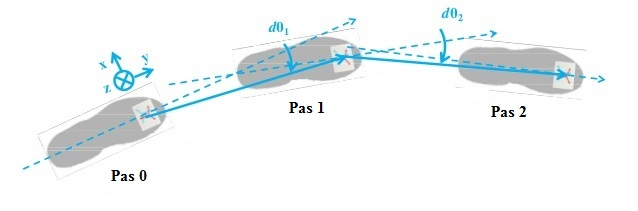
\includegraphics[width=10cm]{figures/pedestrian-dead-reckoning-modified.jpg}
\caption{Descriere vizuală a ideii aplicației}
\label{fig:pdr_idea}
\end{figure}


\subsection{Element de noutate}
\tab{Aplicația implementată aduce ca element de noutate faptul că dispozitivul poate fi ținut în orice poziție relativ la Pământ, cu mențiunea că trebuie să rămână relativ fix în raport cu utilizatorul.}\\

Aplicațiile anterioare restricționau utilizatorul la ținerea dispozitivului într-o poziție nu prea comodă, orizontală în raport cu Pământul.

Tot ca element de noutate este și pasul de calibrare, făcut fie într-un spațiu în care să existe semnal GPS, fie prin introducerea înalțimii utilizatorului. Acest pas de calibrare este folosit pentru a inițializa variabile specifice utilizatorului, astfel încât aplicația să recunoască mișcările acestuia cât se poate de bine.


\subsection{Prezentarea pe scurt a capitolelor}
\tab{În secțiunea \ref{AplicatiiCercetariSimilare} vor fi descrise articole și aplicații ale căror influență se găsește și în lucrarea de față. Vor fi prezentate lucrări de master și de doctorat, articole științifice și aplicații. Acestea au servit ca puncte de sprijin pe toată durata elaborării acestei lucrări, oferind referințe multiple și idei de rezolvare.}

În secțiunea \ref{Teorie} va fi prezentată pe scurt teoria privitoare la senzorii folosiți: GPS, accelerometru, giroscop, magnetometru.

În secțiunea \ref{DetaliiAndroidOS} va fi prezentată platforma pe care se va lucra, Android. Se vor da informații privitoare la istoricul acestei platforme și la modul în care lucrează senzorii.

În secțiunea \ref{ObiecteAndroid} vor fi prezentate obiectele Android care au fost folosite predominant în dezvoltarea aplicației. Se va trece prin componentele unei aplicații Android, precum și prin câteva detalii privitoare la API-ul Google Maps.

În secțiunea \ref{DescriereAplicatie} va fi prezentată pe larg aplicația, începând cu interfața vizuală și finalizând cu partea care rulează în fundal.
%TODO: Ofera mai multe informatii, eventual pe subsectiuni

În secțiunea \ref{TestareAplicatie} vor fi prezentate rezultatele experimentale. Va fi și locul în care vom explica metodologia de testare.

În secțiunea \ref{Discutii} vor fi analizate rezultatele secțiunii de testare și se va încerca găsirea unor explicații relativ la rezultate. Tot în această secțiune vor fi descrise și ideile de îmbunătățire a aplicației.

În secțiunea \ref{Concluzii} va fi concluzionată munca efectuată.

\newpage


\section{Muncă anterioară} \label{AplicatiiCercetariSimilare}
%Pagini in care se prezinta cercetarile si aplicatiile anterioare
%In prima parte se prezinta cercetarile
%In a doua parte se prezinta aplicatiil
Domeniul navigației cu ajutorul senzorilor este unul în care se fac studii intense datorită impactului pe care îl poate avea. Putem găsi utilizări în industrii precum cea automotive, în zona de vânzări produse, în zona medicală sau ca ajutor pentru echipe de salvare.

În studiul pentru elaborarea acestei lucrări am citit studii precedente, axate pe diferite componente ale aplicației pe care vreau să o dezvolt. Sunt cercetări în zona detecției pașilor cât mai corect, în zona determinării lungimii parcurse cu fiecare pas sau chiar în partea de hărți și orientare.

Pe lângă studiile citite, am încercat să găsesc și aplicații similare cu care să compar munca mea. Aceste aplicații mi-au oferit, pe lângă posibilitatea de a mă compara cu ceva, și idei pe care să la folosesc în propria implementare.

O să încep cu cercetările existente deoarece consider că acestea stau la baza ulterioarelor dezvoltări de aplicații.

\subsection{Cercetări similare existente}
Dacă este să analizăm munca de cercetare făcută, a cărei rezultat nu a fost o aplicație publicată, trebuie să luăm în considerare câteva articole care explică diferite metode de a obține ce se dorește și prin această lucrare.

Aceste articole au fost publicate de echipe întregi, cu acces la finanțare și la tehnică. Acele articole care nu au fost făcute în echipă au fost făcute ca lucrări de master sau chiar de doctorat. %TODO: Modificare daca nu e asa%

Dintre sursele pe care le consider relevante și de la care am învățat vreau să enumăr:
 
\begin{itemize}  
\item \textbf{Dead Reckoning Algorithms for Indoor Localization} \cite{ZhangYu}:\\
Această lucrare este teza de masterat a singaporezului Zhang Yu și a reprezentat un punct de sprijin în elaborarea lucrării mele, atât prin informațiile oferite de el, cât și prin bibliografia extinsă pe care a prezentat-o. În bibliografia lui am găsit alte articole extrem de interesante din care am luat idei.

În teza sa de master, el a încercat să compare robustețea unui număr de algoritmi de dead reckoning pentru persoane, folosind senzorii unei tablete. Diferența este că el face procesarea offline, nu pe dispozitiv. Aplicația pe care eu doresc să o propun face procesarea în timp real.

Algoritmii prezentați de acesta variază de la algoritmi bazați pe \textbf{triangularizare folosind Wi-Fi} până la \textbf{Filtre Kalman Extinse}. Este de interes și studiul capabilităților senzorilor făcut de către Zhang Yu. De asemenea, principiile detecției pașilor au fost de mare ajutor.

\item \textbf{A Step, Stride and Heading Determination for the Pedestrian
Navigation System} \cite{StepLengthAndHeadingDetermination}:\\
Această lucrare prezintă principiile de bază ale detecției pașilor, determinării lungimii unui pas și a orientării. Este o lucrare cu o analiză destul de detaliată a mersului uman, din care se extrag metode experimentale de determinare a pașilor.

\item \textbf{Using the ADXL202 in Pedometer and Personal Navigation Applications} \cite{HarveyWeinberg}:\\
Acest scurt articol prezintă o formulă de calculare a distanței parcurse într-un pas.

Formula estimează lungimea unui pas k, $\rho_{k}$, ca fiind $\rho_{k} = K \sqrt[4]{A_{max}^{(k)} + A_{min}^{(k)}}$, unde $A_{max}^{(k)}$ este valoarea maximă a accelerației în timpul celui de-al k-lea pas, $A_{min}^{(k)}$ este valoarea minimă a accelerației în timpul celui de-al k-lea pas, iar $K$ este o constantă dependentă de utilizator. Această constantă se va afla printr-o procedură de calibrare.

Această formulă este ulterior demonstrată ca fiind una bună în practică de către Diego Alvarez și colegii săi în articolul „Comparison of step length estimators from wearable accelerometer devices” \cite{StepLengthEstimatorsComparaison}.

\item \textbf{An Indoor Navigation System For Smartphones} \cite{AbhijitChandgadkar}:\\
În această lucrare se prezintă o modalitate de a oferi navigație în interiorul clădirilor, similar lucrării noastre. Aceasta se bazează pe aceeași idee de a estima poziția pe baza distanței parcurse cu fiecare pas și a diferențelor de orientare. 

Se introduce și o metodă de reducere a erorilor prin folosirea unor marcaje amplasate în puncte cheie ale clădirii. Pentru aplicația noastră nu este fezabil un plan similar deoarece nu există o clădire țintă, ci se dorește funcționarea în orice clădire.

De asemenea, aplicația implementată în această lucrare își propune să funcționeze în orice mediu fără semnal, nu doar în clădiri.

\item \textbf{Exploring Smartphone-Based Indoor Navigation: A QR Code Assistance-Based Approach} \cite{QRNavigation}:\\
În acest articol este prezentată o metodă de navigație similară celei implementate în această lucrare. 

Pentru reducerea erorilor autorii propun montarea unor marcaje cu coduri \textbf{QR} (Quick Response) în puncte cheie ale clădirii. La fel ca mai sus, nu este fezabilă o astfel de abordare decât atunci când există clădiri țintă în care aplicația va fi folosită.

\item \textbf{Filtering and Tracking for a Pedestrian Dead-Reckoning System} \cite{SuratKwanmuang}:\\
În această lucrare de doctorat se implementează un sistem capabil să urmărească mișcările unui om pentru ca mai apoi un robot să poată urma o aceeași traiectorie. Motivația din spatele acestei idei este aceea de a avea un robot care să care provizii sau materiale grele în locul omului. Această aplicație are potențiale implicații în zona militară.

Deși se implementează un dead reckoning pe bază de filtru Kalman, aplicația are un mare dezavantaj, acela că limitează utilizatorul la purtarea senzorului fixat pe picior. Această limitare face ca aplicația să nu fie utilă în zona în care dorește să intre aplicația prezentată în această lucrare de licență, aceea de a avea navigație pe dispozitive deja disponibile, fără a fi nevoie de alți senzori.

\item \textbf{Filtering and Tracking for a Pedestrian Dead-Reckoning System} \cite{SDCPA10b} și \textbf{Indoor pedestrian navigation system using a modern smartphone} \cite{SCM10}:\\
Aceste articole stau la baza implementării unei aplicații la \textbf{CRS4} (Center for Advanced Studies, Research and Development in Sardinia) a unei aplicații, \textbf{Roodin}. Această aplicație are la bază o idee similară aplicației prezentate în această licență.

\item \textbf{Pedestrian localisation for indoor environments} \cite{OliverWoodman}:\\
În teza sa de doctorat, Oliver Woodman prezintă metode de a obține navigație în interiorul clădirilor folosind senzori. Explicațiile sale cu privire la senzori și la ce înseamnă un sistem de navigație inerțială sunt importante pentru a înțelege eventualele surse de eroare.

Prezentarea sa ajunge la disuții privitoare la filtre posibile care să îmbunătățească acuratețea (cum ar fi filtre Bayes sau filtre Kalman).

Totuși, implementarea sa se bazează pe folosirea unor senzori externi, montați pe picior, ceea ce limitează aplicabilitatea sa.

\end{itemize}


\subsection{Aplicații similare existente}
În încercarea de a oferi sisteme de navigație rezistene la erori sau la lipsa semnalului s-au construit mai multe aplicații similare cu cea din această lucrare.

Aceste aplicații fie încearcă îmbunătățirea semnalului GPS prin adăugarea măsurătorilor de la senzori, fie încearcă să ofere posibilitatea navigării exclusiv folosind senzorii, fie ei senzorii descriși în unul din capitolele anterioare, fie ei camera telefonului sau chiar Wi-Fi-ul.

Am putea considera aplicații similare și acele aplicații care încearcă oferirea de noi informații utilizatorilor folosind date de la GPS și senzori, de exemplu pentru a găsi poziția și respectiv orientarea lor în raport cu eventuale puncte de interes.

\begin{itemize}  
\item \textbf{Google Maps} \cite{GoogleMaps}:\\
Dacă discutăm despre aplicații despre navigație pentru pietoni, nu putem omite poate cea mai cunoscută dintre ele, Google Maps. Această aplicație este oferită de către Google și oferă funcționalități de bază, cum ar fi afișarea locației curente, oferirea de indicații către alte locații, dar și afișarea de informații legate de mijloacele de transport în comun sau starea traficului. Este o aplicație care arată cât de multe date are Google la dispoziție. 

Marele dezavantaj al acestei aplicații este acela că are nevoie de acces la semnal GPS și la serviciul de date pentru descărcarea hărților (se oferă acum posibilitatea descărcării hărților pentru ca aplicația să funcționeze și offline).
 
Google Maps este inutil în zonele cu semnal GPS slab sau în interiorul clădirilor. Nu îl putem folosi, de exemplu, pentru a găsi o sală de curs într-o facultate, un cabinet într-un spital sau un magazin într-un mall. 
 
\item \textbf{Strava} \cite{Strava}:\\
O altă aplicație care oferă navigație pentru pietoni, și nu numai, este Strava. Această aplicație a fost construită ca un asistent de fitnes folosit pentru a înregistra traseele celor cărora le place să facă sport, însă componenta sa socială permite salvarea de trasee și oferirea/parcurgerea lor.

Deoarece este în principal o aplicație de fitness, Strava nu pune mare accent pe parte de navigație. Nu găsim în Strava informațiile pe care le găsim în Google Maps. Pe lângă acest dezavantaj, și Strava suferă de aceeași problemă a dependenței de GPS. Fără GPS aplicația doar măsoară numărul de pași și estimeasă distanța parcursă.

\item \textbf{SmartNavi - Step Navigation} \cite{SmartNavi}:\\
O aplicație care se apropie de ceea ce se dorește a fi această lucrare este SmartNavi - Step Navigation. Această aplicație a fost creată în cadrul unui set de experimente pentru platforma Android, prin care Google a oferit posibilitatea unor dezvoltatori să își pună ideile în practică, aceștia beneficiind de marketingul făcut de compania gigant. Prin participarea la aceste experimente, dezvoltatorii sunt de acord să facă public codul sursă pentru a putea fi folosit și de către alți dezvoltatori care să ducă mai departe ideile și să lanseze aplicații noi.

Aplicația oferă posibilitatea de a oferi navigație fără a avea semnal GPS, doar pe baza măsurării numărului de pași și a direcției luate de utilizator. Aceste este un mare avantaj dacă o comparăm cu aplicații precum Google Maps sau Strava. Aplicația recunoaște pașii și direcția bazându-se pe senzorii dispozitivului. 

Pe lângă oferirea de navigație, aplicația poate să se comporte ca un furnizor de locație, care poate fi util pentru alte aplicații din sistem. 

Dezavantajul acestei aplicații este că utilizatorul trebuie să țină mereu telefonul în fața lui (deși poziția este una normală pentru situația în care trebuie să urmărească indicațiile de pe ecran, pot exista situații în care utilizatorul să dorească să țină telefonul în altă poziție).

SmartNavi dorește să ofere posibilitatea de a avea navigație fără un consum foarte mare de baterie, dorința lor nu este neapărat de a oferi un sistem capabil de a lucra în interiorul clădirilor. Acesta poate fi privit ca un dezavantaj, aplicația nu are o țintă clară, ea doar dorește să arate ce este posibil pe această platformă.

\item \textbf{DaRe - Pedestrian Navigation} \cite{DaRe}:\\
Aplicația DaRe oferă navigație primind date de la un senzor montat pe piciorul purtătorului, care comunică prin Bluetooth cu smartphone-ul. DaRe are două moduri de lucru: metoda grafică, în care afișează traseul pe un plan bi-dimensional, și modul text, în care afișează date cum ar fi: numărul de pași, distanța parcursă și viteza medie. 

Totuși, comparativ cu aplicația descrisă în această lucrare, DaRe are marele avantaj de a avea un senzor extern plasat exact pe piciorul purtătorului. Asta garantează că pașii vor fi detectați aproape perfect, comparativ cu detecția făcută cu ajutorul telefonului. Măsuratorile făcute cu telefonul sunt predispuse la mișcările utilizatorului, care pot să declanșeze detectorul de pași și să numere în plus.

Un alt dezavantaj al DaRe este acela că nu plasează utilizatorul pe o hartă, ci doar îl arată într-un plan bidimensional simplu. Aplicația nu are decât scop de testare al posibilităților unui astfel de sistem.

\item \textbf{Landmarker} \cite{Landmarker}:\\
O altă aplicație care se bazează foarte mult pe senzori și pe locație pentru a oferi utilizatorului informații este Landmarker. Această aplicație dorește să aducă pe platforma Android un mod nou de a găsi puncte de interes în orașe. 

Aplicația recunoaște poziția curentă a utilizatorului și, folosind senzorii dispozitivului, reacționează la mișcările acestuia, arătându-i pe ecran unde (distanța și punctul cardinal) se află locațiile de interes.

Landmarker intră într-o altă zonă față de toate celelalte aplicații, aceea a oferirii de informații legate de puncte de interes din apropiere. Nu se ocupă de oferirea de navigație (ba chiar oferă posibilitatea să se treacă la Google Maps dacă se dorește a se găsi un traseu până la punctul de interes) și este dependentă de GPS. Este interesantă în contextul lucrării curente deoarece folosește senzorii telefonului pentru a determina orientarea față de un punct cardinal, ceea ce este esențial pentru oferirea de navigație în clădiri sau zone cu semnal GPS slab.

\item \textbf{Maps People} \cite{MapsPeople}:\\
Aceast serviciu oferă componenta lipsă a oricărei aplicații de navigație în interiorul clădirilor, adică partea de hărți. Este un serviciu cu plată care permite căutarea de locații, oferirea de anunțuri relevante și de rute între locații.

\end{itemize}

\newpage



\section{Teorie} \label{Teorie}
%Pagini in care este descrisa teoria din spatele aplicatiei
%In prima parte se prezinta teoria din spatele GNSS
%In a doua parte se prezinta teoria din spatele senzorilor

În următoarele pagini se va face o trecere prin detaliile teoretice legate de localizarea prin satelit, dar și a modului de lucru al senzorilor: accelerometru, giroscop, magnetometru.

\subsection{Teoria din spatele GNSS}
\textbf{Localizarea} se face în zilele noastre cu ajutorul sistemului global de navigație, numit \textbf{GNSS} (Global Navigation Satellite System). Aceste este, așa cum lasă și numele său să se înțeleagă, acesta este un sistem de sateliți aflați în spațiu care transmit date către module capabile să le înțeleagă, aflate aici, pe Pământ.

Construirea acestui sistem a început în anii '60, prin lansarea de către \textit{Departament of Defence} a a primilor sateliți, cu scopul de a cunoaște locația submarinelor care transportau focoase nucleare. În anii '70
armata americană voia un sistem de sateliți care să ofere navigație robustă. Folosindu-se de „efectul \textbf{Doppler}”, receptorul datelor putea să calculeze distanța la care se afla de emițător. Efectul Doppler reprezintă schimbarea frecvenței unei unde pentru un observator care este în mișcare relativ la sursa undei \cite{DopplerEffectWikipedia}. Pentru vizualizarea acestuia, consultați Figura \ref{fig:doppler_effect_moving_object} \cite{DopplerEffectWikipedia}. Săgeata roșie indică direcția în care se deplasează obiectul.

\begin{figure}[h]
\centering
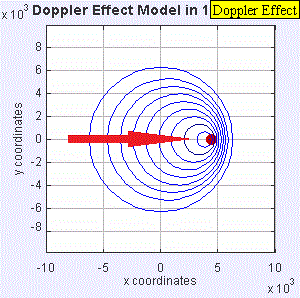
\includegraphics[scale=1]{figures/doppler_effect_moving_object.png}
\caption{Doppler Effect}
\label{fig:doppler_effect_moving_object}
\end{figure}

Combinând datele de la mai mulți emițători, receptorul putea să estimeze poziția sa curentă. Așa cum putem observa în Figura \ref{fig:gps_signals}, preluată din articolul NASA referitor la istoria GPS \cite{GPSHistoryNASA}, locația curentă se estimează într-o zonă foarte probabilă în care se află receptorul. Această zonă nu este însă un punct, ci un volum. Asta înseamnă că oricâți sateliți am avea vizibili, poziția noastră calculată este doar o estimare, deci supusă erorilor.

\begin{figure}[h]
\centering
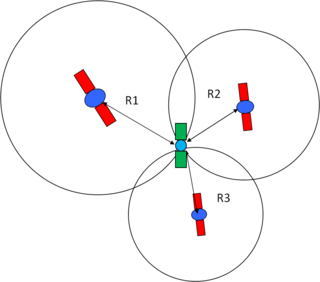
\includegraphics[width=10cm]{figures/gps_signals.png}
\caption{Semanlele radio GPS}
\label{fig:gps_signals}
\end{figure}

Receptorul știe că un anumit satelit transmite un anumit mesaj la un anumit moment în timp. Atunci când primește acel mesaj, receptorul verifică diferența de timp între ora înregistrată de el și ora la care știa că acel mesaj va fi trimis. Cunoscând diferența aceasta de timp el poate calcula distanța la care se află de satelit, deoarece știe și viteza undelor electromagnetice.

Pentru calculul locației curente se pleacă de la un fapt cunoscut, acela că receptorul se află fie pe suprafața Pământului, fie la o distanță mică de acesta (fie în aer sau în ocean).

Cunoscând acest fapt, estimarea locației la nivel de \textbf{latitudine} și \textbf{longitudine} se poate face cu doar \textbf{trei sateliți}. Sunt necesari trei sateliți deoarece unul dintre aceștia va juca rolul de satelit care oferă timpul de referință, iar ceilalți doi vor fi folosiți pentru a estima două sfere în care receptorul este cel mai probabil să se afle. Intersecția acelor două sfere va fi, în condițiile date, un punct sau maxim două puncte. Unul dintre acele puncte se va afla pe Pământ și celălalt în spațiu sau mult în interiorul Pământului (către centrul său). Receptorul GPS va ști să aleagă punctul aflat pe Pământ.\\

Pentru estimarea locației la nivel de \textbf{latitudine}, \textbf{longitudine} și \textbf{altitudine}, mai este necesar încă un satelit.

Cu cât sunt mai mulți sateliți vizibili, cu atât este mai precisă estimarea poziției. De aceea, atunci când s-au proiectat constelațiile de sateliți s-a avut în vedere prezența unui număr de minim trei sateliți deasupra oricărui punct de pe Pământ, la orice oră.\\

Cunoscând acum modul în care se face localizarea cu ajutorul sateliților, trebuie să vedem ce anume cauzează probleme.

Prima mare problemă este acuratețea sistemului în sine. Conform Tabelului \ref{tab:accuracy_table}, nicio constelație nu garantează acuratețe mai mare de $10m$.

\begin{table}[h]
\centering
    \begin{tabular}{ | l | l | l | l | l | l |}
    \hline
    \textbf{Constelație} & GPS & GLONASS & GALILEO & BEIDOU & QZSS \\ \hline
    \textbf{Acuratețe ($m$)} & $7.8m$ \cite{GPSAccuracy} & $ 4.5–7.4m$ \cite{GLONASSAccuracy} & $?m$ & $10m$ \cite{BeiDouAccuracy} & $?m$ \\ \hline
    \end{tabular}
    
    \caption{Acuratețea declarată a constelațiilor în $95\%$ din situații}
    \label{tab:accuracy_table}
\end{table}

A doua problemă stă în erorile datorate receptoarelor GPS. Acestea sunt de dimensiuni foarte mici, pentru a încăpea în telefoane mobile și sunt foarte aproape de eventuale perturbații magnetice. Acestea duc la capabilități mult reduse, ceea ce înseamnă estimări eronate. Antene de dimensiuni mai mari sunt mult mai eficiente, însă este clar că nu este fezabilă utilizarea acestora.

O altă problemă stă în relieful planetei. Relieful accidentat din munți face ca semnalul să fie reflectat, ceea ce cauzează probleme la partea de recepție, unde putem întâlni cazuri în care să recepționăm semnale cu întârzieri foarte mari. Aceste întârzieri în timp duc la erori de estimare a distanțelor. Dar nu doar relieful natural cauzează probleme, ci și clădirile. Acestea aduc aceleași probleme cu reflexia undelor, pe lângă problema acoperirii cerului vizibil de către receptor, micșorând zona în care acesta poate să vadă sateliți.\\

Deoarece însuși sistemul de navigație este unul predispus erorilor, trebuie încercată îmbunătățirea acestuia. Aceasta se poate realiza fie prin îmbunătățirea stateliților și a receptoarelor, fie prin utilizarea unor senzori care să augumenteze datele de la sateliți.

\newpage
\subsection{Teoria din spatele senzorilor}
În continuare se va face o scurtă trecere prin detaliile legate de câțiva senzori ale căror date pot fi folosite pentru estimare poziției curente. Acești senzori sunt: \textbf{accelerometrul}, \textbf{giroscopul} și \textbf{magnetometrul}.\\

\textbf{Accelerometrul}\\
Accelerometrul este un senzor capabil să măsoare accelerația aplicată asupra sa. Accelerația este rata schimbării vitezei unui obiect. Accelerometrul măsoară rata schimbării în $m/s^{2}$.

Forțele care acționează asupra unui accelerometru pot fi statice sau dinamice. Forțele statice sunt acele forțe constante, cum ar fi gravitația. Forțele dinamice sunt rezultatul mișcării accelerometrului.

Accelerometrul este util în detectarea mișcării. Folosind un astfel de senzor se poate vedea dacă asupra dispozitivului acționează o forță dinamică. Un alt caz în care accelerometrul poate fi util este acela în care dorim să detectăm dacă un dispozitiv este înclinat sau nu în raport cu direcția gravitației. Pentru a face asta, eliminăm forța statică a gravitației și observăm valorile rămase pe fiecare din cele trei axe. Dacă toate sunt 0, atunci înseamnă că dispozitivul este pe direcția gravitației. Dacă avem valori mai mari decât zero înseamnă că dispozitivul este înclinat.

Cu ajutorul unui accelerometru fără erori am putea, cel puțin teoretic, să estimăm distanța parcursă. Pentru a face asta, integrăm de două ori valoarea accelerației în raport cu timpul scurs.

Accelerația reprezintă, așa cum am precizat deja, rata schimbării vitezei unui obiect, deci derivata în raport cu timpul a vitezei. Viteza reprezintă distanța parcursă într-o perioadă de timp, deci derivata distanței în raport cu timpul.

\begin{equation} 
\left.
\begin{aligned} a = \dfrac{dv}{dt}\\ v = \dfrac{dx}{dt} \end{aligned} \right\} \Rightarrow a = \dfrac{d^{2}x}{d^{2}t}
\end{equation}

Cum integrarea este opusa derivării, putem afla distanța parcursă cunoscând accelerația prin aplicarea unei duble integrale.

\begin{equation} 
\left.
\begin{aligned} v = \int_{}^{} a dt\\ x = \int_{}^{} v dt \end{aligned} \right\} \Rightarrow x = \iint_{} a \,dt\,dt
\end{equation}\\


\textbf{Giroscopul}\\
Giroscopul este un senzor capabil să măsoare schimbarea unghiului de rotație în timp (viteza angulară). Viteza angulară este măsurată în $rad/s$.

Giroscopul este util în detectarea rotației, prin integrarea în raport cu timpul. 

Viteza angulară reprezintă, așa cum am precizat deja, rata schimbării poziției angulare în timp, deci derivata poziției angulare în raport cu timpul.

\begin{equation} 
\left.
\begin{aligned} \dot{\theta} = \dfrac{d \theta}{dt} \end{aligned}
\right.
\end{equation} 

Cum integrarea este opusa derivării, putem afla unghiul de rotație cunoscând viteza angulară prin aplicarea unei integrale.

\begin{equation} 
\left.
\begin{aligned} \theta = \int_{}^{} \dot{\theta} dt \end{aligned}
\right.
\end{equation} 

El poate fi folosit în detectarea vibrațiilor produse de factori externi. Giroscoapele sunt extrem de utilizate în robotică, atunci când se dorește ca robotul să fie capabil să își păstreze echilibrul. Această utilizare apare și în zona aviației, acolo unde este necesară păstrarea echilibrului și cunoașterea unghiului de înclinare în lipsa unor alte puncte de referință.

O altă utilizare a giroscopului este în industria automobilelor, acolo unde este folosit pentru algorimul de dead reckoning. Putem găsi giroscoape și în camere foto, pentru corectarea vibrațiilor.

În zona distracției, giroscopul este folosit în prezent în telefoane mobile pentru a detecta mișcarea dispozitivului.\\

\textbf{Magnetometrul}\\
Magnetometrul este un senzor care măsoară intensitatea câmpului magnetic  pe fiecare dintre cele trei axe de coordonate într-un punct din spațiu. Valorile raportate de magnetometru sunt în $\mu T$ (microTesla).

Magnetometrul este crucial în detectarea orientării dispozitivului în raport cu Polul Nord Magnetic al Pământului.

\newpage
\section{Sistemul de operare Android} \label{DetaliiAndroidOS}
%Pagini in care este descris sistemul de operare Android
\subsection{Despre Android \cite{AndroidHistoryAndroidCentral}} 
Android este un sistem de operare dedicat dispozitivelor mobile, smartphone-uri, smartwatch-uri, precum și TV-urilor sau chiar dispozitive din interiorul automobilelor.

Sistemul de operare Android este bazat pe un kernel de Linux și a fost construit pentru a fi folosit în principal pe dispozitive touchscreen. Este cel mai folosit sistem de operare disponibil pe dispozitive mobile încă din 2013.

Sistemul a fost dezvoltat de către Android Inc., companie fondată în 2003. Dezvoltatorii au avut dorința de a ajuta la construirea de dispozitive mai inteligente, conștiente de locația și preferințele utilizatorilor.

În 2005 compania Android Inc. a fost achiziționată de către Google pentru o sumă de aproximativ 50 milioane de dolari, iar intenția Google era clară pentru mulți, intrarea pe piața dispozitivelor mobile.

La data de 5 noiembrie 2007, un consorțiu de companii precum Google, HTC, Sony, Samsung, T-Mobile, dar și producători de chipset-uri, Qualcomm și Texas Instruments, a fost lansat. Acest consorțiu, numit „Open Handset Alliance”, al cărui scop era de a dezvolta standarde deschise pentru dispozitive mobile, a lansat în aceeași zi sistemul de operare Android, ca prim produs al său.

Primul smartphone cu sistem de operare Android lansat a fost HTC Dream, în luna octombrie a anului 2008.

Fiecare nouă versiune a sistemului este denumită în ordine alfabetică după un desert: „Cupcake”, „Donut”, „Eclair”, „Froyo”, „Gingerbread”, „Honeycomb”, „Ice Cream Sandwich”, „Jellybean”, „Kit Kat”, „Lolipop” și „Marshmallow”. Următoarea versiune este plănuită pentru acest an, deocamdată ea fiind denumită Android N. Google a oferit utilizatorilor posibilitatea să voteze numele.


\newpage
\subsection{Versiunile Android}
%Android 1.0
\tab{\textbf{Android 1.0} \cite{AndroidVersionsHistory}, \cite{AndroidHistory}, \cite{DeveloperAndroid}}\\
Prima versiune a sistemului de operare Android, denumită, deloc pompos, Android 1.0, dădea impresia de produs nefinalizat, însă lăsa să se întrevadă planurile Google pentru această platformă. Această versiune deja avea părți care, comparate cu ce era  pe piață la momentul acela, erau mult superioare. Sunt lucruri pe care acum le trecem cu vederea, dar care atunci erau noutăți, widget-urile, zonele de notificări și nu numai. 

Prima versiune a Android includea și aplicațiile cu care suntem acum atât de obișnuiți, cum ar fi Gmail sau YouTube. Android Market Beta debuta și ea, oferind posibilitatea de a lista aplicații și jocuri.

Tot în acea perioadă Android și-a câștigat și atât de cunoscutul logo, denumit în interiorul Google „Bugdroid”.\\

%Android Cupcake
\textbf{Android 1.5 - Cupcake \cite{AndroidVersionsHistory}, \cite{AndroidHistory}, \cite{DeveloperAndroid}}\\
Primul mare update al Android-ului a fost versiunea 1.5, denumită, în ceea ce avea să stabilească trendul numelor inspirate din dulciuri, „Cupcake”.

	Lansat în aprilie 2009, Cupcake a fost deschizător de drum pentru dispozitivele cu Android fără tastatură fizică. Telefoanele precedente aveau încorporate și tastaturi fizice, însă cu această versiune de sistem de operare, Google a introdus tastatura virtuală, precum și posibilitatea folosirii de tastaturi third-party.

	Acestea arătau evenimentele și respectiv melodia curentă. Pentru prima dată aplicațiile puteau să își adauge widget-uri proprii. O altă noutate a fost reprezentată de posibilitatea de a roti automat ecranul în funcție de orientarea telefonului, pentru o tranziție ușoară portret-landscape.\\

%Android Donut
\textbf{Android 1.6 - Donut \cite{AndroidVersionsHistory}, \cite{AndroidHistory}, \cite{DeveloperAndroid}}\\
În același an al lansării Android 1.5, Google a lansat și noua versiune, 1.6, numită „Donut”.
	
	Aceasta aducea suport pentru ecrane de diferite rezoluții și densități ale pixelilor, precum și suport nativ pentru comunicarea în banda CDMA (Code Division Multiple Access). Noul sistem oferea și posibilitatea de a efectua căutări, atât în fișierele aflate pe telefon, cât și pe internet, prin așa numitul „Quick Search Box”. Tot cu această versiune a venit și posibilitatea de a vedea consumul de baterie al dispozitivului.
	
	Android Market a fost refăcut pentru a putea expune aplicațiile gratuite de top, precum și aplicațiile de top plătite, în contextul exploziei de noi aplicații de pe această platformă. Pentru prima dată au fost introduse și butoane care ofereau acces facil la setări precum Wi-Fi, Bluetooth, GPS, Sincronizare sau Luminozitate.\\

%Android Eclair
\textbf{Android 2.0, 2.0.1, 2.1 - Eclair \cite{AndroidVersionsHistory}, \cite{AndroidHistory}, \cite{DeveloperAndroid}}\\
Lansat în octombrie 2009, Android 2.1, denumit și „Eclair”, a adus câteva îmbunătățiri precum: posibilitatea de a căuta în toate SMS-urile și MMS-urile salvate pe telefon, viteză de tastare mărită pentru tastatura virtuală, setări de accesibilitate, calendar, dar și un API pentru VPN (Virtual Private Network). Pentru browser, Android aducea suport HTML5. Tot acum au apărut double-tap-zoom și pinch-to-zoom.
	
	Tot în versiunea Eclair a fost introdusă și posibilitatea de a folosi Google Maps pentru navigație, aceasta oferind indicații pas-cu-pas, dar și informații legate de trafic, caracteristici similare serviciilor de navigație din automobile, cu diferența că cele oferite de Google erau gratuite.

	O altă funcționalitate care acum este extrem de utilizată și a fost adăugată înca din versiunea Eclair este cea de Speech-to-Text, care permitea introducerea de text dictând telefonului.\\
	
%Android Froyo
\textbf{Android 2.2 - Froyo \cite{AndroidVersionsHistory}, \cite{AndroidHistory}, \cite{DeveloperAndroid}}\\
Poate cea mai importantă noutate a acestei versiuni a fost aceea a introducerii mașinii virtuale Dalvik, care oferea Just-in-time Compiling, oferind îmbunătățiri masive ale vitezei Android-ului.

	Cu această versiune a fost oferită și posibilitatea de a instala sau muta aplicațiile pe cardul de memorie pentru a elibera memoria internă a telefonului. Altă noutate a fost reprezentată de hotspot-ul Wi-Fi, care permitea telefonului să ofere Wi-Fi altor dispozitive.

	Browser-ul a cunoscut și el îmbunătățiri ale vitezei prin schimbarea motorului de JavaScript la cel folosit de Chrome, V8.\\

%Android Gingerbread
\textbf{Android 2.3, 2.3.3 - Gingerbread \cite{AndroidVersionsHistory}, \cite{AndroidHistory}, \cite{DeveloperAndroid}}\\
Cu această nouă versiune a Android a apărut și ceea ce avea să devină un nou obicei al Google, acela de a lansa un telefon sub marcă proprie la câteva versiuni de soft distanță. Aceasă linie de telefoane se va numi Nexus și va fi construită cu producători diferiți la fiecare nouă iterație, ea oferind un Android „curat”. Primul telefon din gama Nexus a fost Nexus S, oferit de către Google în parteneriat cu Samsung.

	Sistemul de operare a adus suport pentru NFC (Near Field Communication), pentru ecrane cu rezoluții mari, pentru telefonie via internet (VoIP), dar și îmbunătățiri ale interfeței vizuale.

	Noul garbage collector concurent a adus un spor de viteză. A fost mărită și viteza de distribuție a evenimentelor în sistem. Tot cu această versiune s-a adăugat și suport nativ pentru mai mulți senzori (cum ar fi giroscopul și barometrul), suport pentru multiple camere video, dar și posibilitatea efectuării de apeluri video.

	Pentru dezvoltatori a fost îmbunătățit suportul pentru scrierea de cod nativ și s-au introdus API-urile pentru jocuri.\\

%Android Honeycomb
\textbf{Android 3.0 - Honeycomb \cite{AndroidVersionsHistory}, \cite{AndroidHistory}, \cite{DeveloperAndroid}}\\
Această nouă versiune a fost lansată cu scopul de a îmbunătăți experiența de utilizare a sistemului pe tablete. Pe lângă îmbunătățirile aduse la nivelul interfeței grafice, au fost aduse și îmbunătățiri la nivelul suportului pentru procesoare multi-core.

	A fost introdus și API-ul pentru utilizarea Fragmentelor, care permiteau dezvoltatorilor de aplicații sa folosească suprafața mai mare a ecranului unei tablete pentru a afișa mai multe părți ale aplicației. Folosirea Fragmentelor permitea separarea aplicațiilor pentru telefoane de cele pentru tablete într-un mod foarte simplu: dacă exista suficient spațiu, se afișau mai multe fragmente ale aplicației, altfel se afișa doar unul și utilizatorul trebuia să navigheze între acestea.

	A fost introdus și conceptul de Action Bar, adică acel spațiu din partea superioară a unei aplicații similar unui meniu dintr-o aplicație desktop.\\

%Android Ice Cream Sandwich
\textbf{Android 4.0 - Ice Creak Sandwich \cite{AndroidVersionsHistory}, \cite{AndroidHistory}, \cite{DeveloperAndroid}}\\
Această versiune oferea o experiență unificată smartphone-tabletă, ea înlocuind complet versiunea Honeycomb și aducând noutățile ei și pe smartphone-uri.

	A fost îmbunătățit multitaskingul, notificările au devenit mai bogate, ecranul de start au fost și el modificat pentru a se reduce consumul de spațiu. S-a adăugat un sistem de management al consumului de date.

	Multitaskingul a devenit acum mai vizibil pentru utlizatorul final, acesta putând acum să selecteze aplicația pe care să o redeschidă. Utilizatorul poate vedea o listă de aplicații pe care le-a folosit în ultima perioadă, apoi poate selecta aplicația pe care să o readucă în prim-plan.

	În partea de jos a ecranului au apărut aplicațiile favorite, într-un aranjament similar celui de pe iPhone. Gesturile încep să devină parte esențială a experienței de utilizare a smartphone-ului, ele putând fi folosite pentru a șterge notificări, pentru a schimba tab-urile în browser, dar și pentru a respinge/accepta apeluri.

	Una din inovațiile aduse a fost Android Beam. Acest sistem permitea transferul de date între dispozitive care dispuneau de NFC. Acest transfer se făcea cu viteze mai mari decât ale Bluetooth-ului, într-un mod extrem de facil din perspectiva utilizatorului. Acesta trebuia doar să apropie cele două dispozitive și să apese „Trimitere”.\\

%Android JellyBean
\textbf{Android 4.1, 4.2, 4.3 - Jelly Bean \cite{AndroidVersionsHistory}, \cite{AndroidHistory}, \cite{DeveloperAndroid}}\\
Această iterație a Android a adus noi îmbunătățiri la capitolul viteză prin introducerea „Project Butter”, care implementa Vsync și triple-buffering. Notificările au fost și ele modificate, putând conține acum până la 8 linii de text și chiar butoane la baza lor. Aceste butoane puteau fi folosite pentru a lua acțiuni în funcție de notificare.

	În Android Jelly Bean a fost lansat și Google Now, asistentul virtual al Google. Acesta oferă informații legate de vremea din locația curentă, precum și despre timpii necesari pentru a ajunge între diferite locații.

	Printre noutăți se numără și posiblitatea de a avea mai multe conturi pe același dispozitiv. Tot acum s-a adăugat și suportul pentru ecrane externe, eventual via Miracast (Wi-Fi Display).

	Alte îmbunătățiri sunt date de adăugarea HDR (High Dynamic Range), a Bluetooth Low Energy, dar și a OpenGL ES3.0, care aducea sporuri de performanță la nivel grafic.\\

%Android KitKat
\textbf{Android 4.4 - KitKat \cite{AndroidVersionsHistory}, \cite{AndroidHistory}, \cite{DeveloperAndroid}}\\
Poate cea mai importantă funcționalitate adăugată cu această versiune este cea a interacțiunii cu telefonul prin comenzi vocale. Faimosul „Ok, Google” a fost oferit începând cu această versiune. Tot acum s-au făcut eforturi pentru ca Android să poată rula mai bine pe dispozitive mai slabe din punct de vedere hardware. Acum Android putea rula chiar și pe 512 MB de RAM.

	S-a adăugat și un nou sistem de acces la stocare, care a permis dezvoltatorilor precum Box sau Dropbox să integreze serviciile lor direct cu memoria telefonului, oferind acces facil la documente din locații diferite.

	Au fost imbunătățiți și senzorii, prin reducerea consumului lor de baterie. Android nu  mai trimite notificările imediat cum senzorii observă modificările, ci le stochează până are suficiente.  Acum au fost introduși și senzorii de detectare a pașilor și de numărare a pașilor.\\
	
%Android Lollipop
\textbf{Android 5.0, 5.1 - Lollipop \cite{AndroidVersionsHistory}, \cite{AndroidHistory}, \cite{DeveloperAndroid}}\\
Android Lollipop a fost versiunea în care a apărut noul stil vizual propus de Google, „Material Design”. Acest ghid despre cum trebuie să arate interfața vizuală a aplicației a fost un mare pas către unificarea experienței de utilizare a aplicațiilor de pe această platformă.
	
	Material Design este un set de reguli de design inspirat din modul în care arată hârtia în diferite combinații de lumini și umbre.
Componentele grafice din aplicații erau acum reprezentate într-un mod minimalist, ca și cum ar fi niște colaje de hârtie. Google nu a adus doar recomandările legate de cum trebuie să arate componentele grafice, ci și un întreg set de instrumente noi care să ajute dezvoltatorii.
	
	Android 5.0 a adus și îmbunătățiri de performanță prin adăugarea ART runtime în locul Dalvik. Acum există suport pentru procesoare cu arhitectura pe 64 de biți. S-a adăugat suport pentru OpenGL ES 3.1, care a dus la jocuri mai bogate grafic și mai captivante.
	
	Tot începând cu această versiune Android și-a făcut apariția și în zona TV, prin lansarea Android TV. Android nu s-a oprit însă la zona TV, el apărând și în zona auto, prin Android Auto.\\

%Android Marshmallow	
\textbf{Android 6.0 - Marshmallow \cite{AndroidVersionsHistory}, \cite{AndroidHistory}, \cite{DeveloperAndroid}}\\
Android Marshmallow a introdus un nou sistem de permisiuni pentru aplicații. Acest nou model presupunea ca aplicația să ceară drepturi de la utilizator nu la instalare, ci atunci când îi era necesar. Prin acest nou set de reguli se dorea ca utilizatorii să știe mai clar ce acceptă, deoarece înainte utilizatorii nu erau neapărat atenți la ce acceptau, și puteau exista aplicații care să poată avea acces la mai multe date decât le era necesar. Existau aplicații de genul „Lanternă” care aveau acces la contacte, locație, microfon și cameră. Genul acesta de permisiuni sunt în mod clar un pericol la intimitatea utilizatorilor, iar cu Android 6.0 Google a încercat să îl limiteze.

	O altă componentă a sistemului unde cei de la Google au adus îmbunătățiri este cea a consumului de baterie. Prin adăugarea „Doze” și a „App Standby”, aplicațiile consumă acum mai puțină baterie.

	În Marshmallow s-a adăugat și Now On Tap, un asistent virtual care permite să afli informații fără să părăsești aplicația curentă. Este util atunci când vrei să afli ce reprezintă ceva din aplicația curentă.\\

%Android N
\textbf{Android N \cite{DeveloperAndroid}}\\
O nouă versiune a Android este în dezvoltare acum, aceasta având numele de cod „Android N”. Un nume care să urmeze linia numelor inspirate din produse dulci este în curs de a fi ales, Google oferind utilizatorilor posibilitatea să recomande și să voteze numele.
	
	Versiunea Android N este acum în developer preview. Aceast Android promite îmbunătățiri în 3 zone cheie: performanță, productivitate și securitate.
	
	Modificările nu se vor opri aici, ci vor include, pentru prima dată în Android, suport pentru mai multe ferestre. Android Instant Apps va permite testarea unor aplicații fără ca acestea să fie instalate efectiv pe dispozitiv.\\
	

\newpage
\subsection{Senzorii Android}
Majoritatea dispozitivelor care rulează Android au încorporați diverși senzori. Aceștia sunt folosiți în diferite contexte în timpul folosirii dispozitivului. Scopul senzorilor este să urmărească eventuale schimbări astfel încât sistemul să răspundă în cel mai bun mod cu putință.

	Deși poate nu este evident, impactul senzorilor este major. Faptul că ecranul se închide atunci când apropiem telefonul pentru a vorbi, faptul că putem să ne măsurăm distanțele parcurse, bătăile inimii, faptul că putem să folosim telefonul ca sistem de navigație, toate acestea se datorează folosirii senzorilor.
	
	Android împarte senzorii în mai multe categorii \cite{DeveloperAndroid}, deși tratarea lor se face într-un mod aproape unitar: senzori de \textbf{mișcare}, de \textbf{mediu}, de \textbf{poziție} și de \textbf{locație}.

	Încă un mod în care Android împarte senzorii este acela că senzorii pot fi \textbf{hardware} sau \textbf{software}.\\
	
\subsubsection{Sistemul de coordonate al senzorilor}
În general Android folosește un sistem de coordonate standard, cu 3 axe. Valorile venite de la senzori reprezintă schimbările pe aceste trei axe.

Sistemul de coordonate este definit în raport cu ecranul dispozitivului (ținut în pozitie verticală), astfel: axa $X$ este orizontală și orientată către dreapta, axa $Y$ este verticală si orientată către partea superioară a dispozitivului, iar axa $Z$ este axa care „iese” din centrul ecranului. Pentru o referință vizuală se poate consulta Figura \ref{fig:axis_device}, conformă cu documentația Android \cite{DeveloperAndroid}.

\begin{figure}[hbtp]
\centering
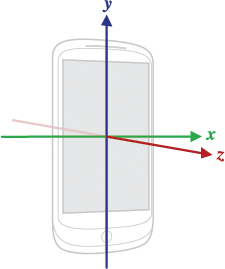
\includegraphics[width=5cm]{figures/axis_device.png}
\caption{Sistemul de coordonate}
\label{fig:axis_device}
\end{figure}


\subsubsection{Senzori de mișcare}
Acești senzori oferă posibilitatea monitorizării mișcării dispozitivului, de exemplu rotație, scuturare, înclinare sau legănare. Doi dintre acești senzori sunt mereu senzori fizici: \textbf{accelerometrul} și \textbf{giroscopul}. Ceilalți trei senzori pot fi atât hardware, cât și software: senzorul de \textbf{gravitație}, cel de \textbf{accelerație liniară} și \textbf{senzorul vectorului de rotație}. Recent au fost adăugați și senzori de \textbf{detectat}, respectiv \textbf{numărat pași}.

	\textbf{Accelerometrul} determină accelerația aplicată dispozitivului prin măsurarea forțelor aplicate senzorului în sine. Totuși, în aceste măsurători intră mereu în calcul gravitația.

	\textbf{Senzorul de gravitație} oferă un vector 3-dimensional care indică direcția și magnitudinea gravitației.

	\textbf{Senzorul de accelerație liniară} oferă un vector 3-dimensional care indică accelerația pe fiecare axă, excluând gravitația.

	Putem formaliza relația dintre accelerații astfel:
	$A_{liniara} = A - g$.\\

	\textbf{Giroscopul} măsoară viteza angulară în raport cu axele $X$, $Y$, $Z$. Viteza angulară este măsurată în $rad/sec$.\\

	\textbf{Senzorul vectorului de rotație} reprezintă orientarea dispozitivului ca fiind combinația dintre o axă și un unghi. Dispozitivul este rotit în jurul uneia dintre axele $X$, $Y$, $Z$ cu un unghi $\theta$. Cele trei componente ale vectorului de rotație sunt: $(x \sin{\theta}, y \sin{\theta}, z \sin{\theta})$. 
	
	Comparativ cu ceilalți senzori de mișcare, acest senzor are valorile exprimate într-un alt sistem de coordonate, unul „global”.
	Acest sistem are următoarele caracteristici:
	\begin{itemize}
	\item $X$ este definit ca fiind tangent la pământ în locația curentă și orientat către Est,
	\item $Y$ este definit ca fiind tangent la pământ în locația curentă și orientat către Polul Nord Magnetic,
	\item $Z$ este definit ca fiind perpendicular la planul definit de $X$ și $Y$, orientat către cer.
	\end{itemize}
	
	Referința vizuală a acestei descrieri este în Figura \ref{fig:axis_globe}, conformă cu documentația Android \cite{DeveloperAndroid}.

\begin{figure}[h]
\centering
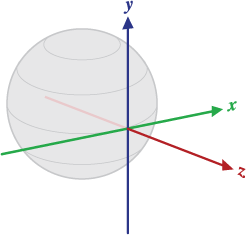
\includegraphics[width=5cm]{figures/axis_globe.png}
\caption{Sistemul de coordonate utilizat de senzorul vector de rotație}
\label{fig:axis_globe}
\end{figure}

\subsubsection{Senzori de mediu}
Acești senzori permit monitorizarea unor valori precum \textbf{umiditatea}, \textbf{intensitatea luminoasă}, \textbf{presiunea atmosferică} sau \textbf{temperatura mediului} din apropierea dispozitivului. Toți senzorii menționați sunt hardware.

Senzorii de \textbf{intensitate luminoasă}, \textbf{presiune atmosferică} sau \textbf{temperatură} sunt unii dintre cei mai simplu de utilizat deoarece nu este necesar ca datele lor să fie corectate. Ei oferă valori cu următoarele unități de măsură: $lx$ (lux) pentru intensitatea luminoasă, $mbar$ (milibar) pentru presiunea atmosferică, respectiv $\celsius$ (grade Celsius) pentru temperatură.

Senzorul de \textbf{umiditate} este și el simplu de folosit. Valorile oferite de el sunt procente.


\subsubsection{Senzori de poziție}
Acești senzori permit monitorizarea poziției dispozitivului într-un cadru de referință global, prin urmărirea schimbărilor de \textbf{câmp magnetic} sau a \textbf{orientării}. Un alt senzor care face parte din această categorie este și  \textbf{senzorul de proximitate}.

\textbf{Senzorul de câmp magnetic} arată fluctuațiile câmpului magnetic al Pământului pe cele trei axe. El oferă valori a căror unitate de măsură este $\mu$T (microTesla). În mod uzual datele de la acest senzor nu sunt folosite în forma lor brută, ci în combinație cu alte date. De exemplu, datele sale, împreună cu cele venite de la accelerometru, pot fi folosite pentru a obține matricile de rotație și de înclinație. Aceste matrici pot fi foloste pentru a se obține \textbf{azimutul}. Azimutul este unghiul la care suntem față de Polul Nord Magnetic. După declinarea magnetică acest unghi ajunge să arate diferența față de Polul Nord, acționând similar unei busole.

\textbf{Senzorul de orientare} permite monitorizarea poziției relative a dispozitivului în raport cu sistemul de coordonate global. Acest senzor face fuziunea descrisă mai sus, combinând datele de la magnetometru și de la accelerometru pentru a obține \textbf{azimutul} (gradele de rotație în jurul axei $Z$), \textbf{pitch}-ul (gradele de rotație în jurul axei $X$) și \textbf{roll}-ul (gradele de rotație în jurul axei $Y$). Deoarece combinarea datelor de la ceilalți doi senzori consumă foarte mult, precizia senzorului este diminuată. De aceea, acest senzor a fost declarat depășit și Android recomandă utilizarea metodei prezentate mai sus pentru obținerea orientării (via matricile de rotație și înclinație).

\textbf{Senzorul de proximitate} raportează cand telefonul este „aproape” sau „departe” de un alt obiect. În mod uzual distanța începând cu care un obiect este considerat apropiat/depărtat este de 5 $cm$.

\subsubsection{Senzori de locație}
Acești senori primesc date despre locația curentă a dispozitivului. Locația curentă poate fi obținută din mai multe surse, cu erori mai mici sau mai mari. Printre surse numim: \textbf{GPS}-ul, \textbf{Wi-Fi}-ul sau chiar datele de \textbf{celulă telefonică}. Pe lângă erorile ce pot veni din faptul că avem de a face cu multiple surse, nici datele provenite din aceeași sursă nu sunt cele mai precise.

Android oferă aplicațiilor acces la servicii de localizare în funcție de ce este disponibil pe dispozitiv. API-ul pentru locație este puțin diferit față de cel pentru ceilalți senzori.\\

Deși acești senzori sunt recunoscuți de către Android, nu este obligatoriu ca toți să fie prezenți și pe dispozitiv. Android nu impune ce senzori să fie prezenți pe dispozitive, ei doar recomandă prezența unora de bază pentru o utilizare cât mai apropiată de cea normală. Producătorii de dispozitive pot la fel de bine să mai adauge senzori noi, nici acest lucru nu este îngrădit de modul de lucru al Android. Fiind open-source, i se poate adăuga suport destul de ușor pentru senzori noi.

\newpage

\section{Obiecte si API-uri Android} \label{ObiecteAndroid}
%Pagini in care sunt descrise obiectele Android, precum si API-urile
Sistemul de operare Android oferă o platformă bogată pentru a permite dezvoltarea de aplicații. Aplicațiile Android sunt scrise în Java. Pe lângă \textbf{Java}, se poate utiliza și \textbf{C++}, prin includerea \textbf{NDK} (Native Development Kit).

Modul în care aplicațiile Android sunt structurate diferă comparativ cu modul „uzual” (al aplicațiilor desktop). Aplicațiile sunt alcătuite din mai multe componente: \textbf{activități}, \textbf{servicii}, \textbf{content provider}, \textbf{broadcast receiver}, fiecare dintre ele putând fi invocată în orice moment. Astfel aplicațiile pot avea mai multe puncte de intrare, câte unul pentru fiecare activitate componentă.

Comunicarea între aceste componente se face folosind alte obiecte specifice Android, \textbf{intent}-urile. Un intent este modul prin care o componentă „spune” ce dorește să facă: să pornească o altă componentă, să ceară deschiderea aplicației standard pentru a afișa conținut, să transmită parametri și nu numai.

O altă componentă esențială a unei aplicații Android este \textbf{manifestul}. Acest fișier XML este folosit pentru a descrie ce componentă trebuie pornită prima dată, care sunt componentele aplicației, ce permisiuni cere aplicația, care este API-ul minim suportat de aplicație, descrie funcționalități hardware sau software pe care aplicația le folosește (acces la Bluetooth, la cameră, etc.)

Pentru stocarea de date Android oferă posibilitatea folosirii unor obiecte de sistem numite \textbf{SharedPreferences}. Acestea stochează datele într-un format XML, similar unui dicționar dintr-un limbaj de programare, în modul cheie-valoare. Pe lângă SharedPreferences se mai pot utiliza și bazele de date SQLite sau fișiere pe stocarea dispozitivului.

Înainte de a continua cu explicarea fiecărei componente, vom descrie succint cum se construiește și cum se rulează o aplicație. Pentru a construi o aplicație, Android pune la dispoziție unelte prin \textbf{SDK} (Software Development Kit). Aplicațiile sunt construite într-un \textbf{pachet Android} a cărei extensie este .apk. Un .apk conține tot ce este necesar aplicației pentru a rula. Fiecare aplicație rulează în izolare, în propria sa mașină virtuală. Fiecare aplicație rulează ca un proces Linux. Android pornește acest proces atunci când se cere deschiderea aplicației și îl închide atunci când fie utilizatorul închide aplicația, fie sistemul are nevoie de resursele consumate de aplicație și aceasta nu este folosită.

\newpage
\subsection{Componentele unei aplicații}
Așa cum am amintit deja, există patru tipuri de componente: \textbf{activități}, \textbf{servicii}, \textbf{content provider}, \textbf{broadcast receiver}.\\

\textbf{Activități}\\
O activitate este o componentă a unei aplicații care oferă un ecran prin care utilizatorul să interacționeze cu ea. Fiecare activitate primește o fereastră pe care să deseneze elementele sale grafice.

Pentru a crea o activitate este necesar să fie creată o clasă care să extindă clasa de bază Activity. Prin aceasta ni se va cere să implementăm metoda onCreate(). Această metodă este entry-point-ul în activitate, similar unui main().

Pentru a trata diferite situații posibile în ciclul de viață al activității este necesar să implementăm metode de tip callback prin care Android să ne notifice. Astfel putem primi notificare când suntem opriți, cand am fost readuși în focus, etc. Ciclul de viață al unei activități este prezentat în Figura \ref{fig:activity_lifecycle}, așa cum apare ea în documentația Android \cite{DeveloperAndroid}.

\begin{figure}[h]
\centering
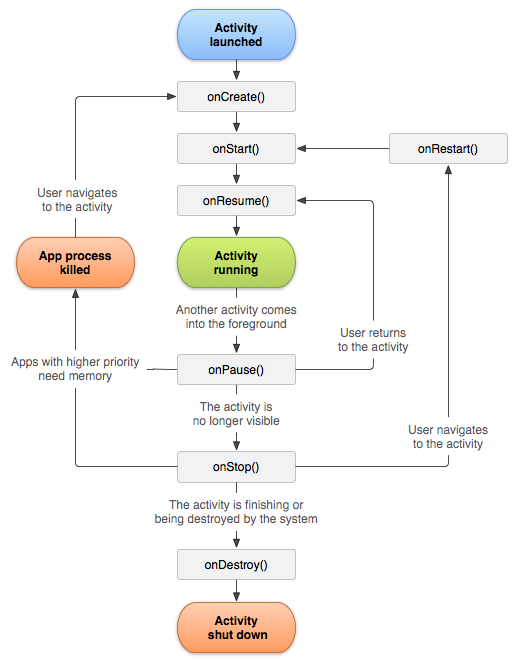
\includegraphics[width=10cm]{figures/activity_lifecycle.png}
\caption{Ciclul de viață al unei activități}
\label{fig:activity_lifecycle}
\end{figure}

Fiind componente prin care utilizatorul poate interacționa cu aplicația, o activitate trebuie să ofere un layout în care să își declare componentele grafice. Acest lucru se face prin scrierea unui XML în care să fie descrisă structura elementelor. Există mai multe modalități de așezare a elementelor grafice pe ecran, iar acestea poartă numele de layout-uri. Amintim: LinearLayout, RelativeLayout, GridLayout, CardLayout, dintre cele mai folosite. Pe lângă layout, este necesar să adăugăm și componente precum butoane sau input-uri. Android are o paletă largă de astfel de elemente, iar unde biblioteca standard nu are elemente se poate interveni fie cu cod propriu, fie cu biblioteci externe.

Dacă se dorește un mod de afișare mai dinamic, se pot adăuga \textbf{Fragmente}.

Un \textbf{Fragment} reprezintă o componentă modulară a unei activități. O activitate poate conține mai multe fragmente care să interacționeze între ele. Este ca și cum am construi o aplicație desktop cu mai multe ferestre disponibile, doar că aici nu avem ferestre efective, ci zone din activitate. Activitatea descrie în layout unde trebuie așezat fiecare fragment iar apoi poate modifica din cod așezarea acestora pentru a crea un comportament dinamic. Putem avea pe o aceeași activitate două ecrane și să ajungem de la unul la celalalt printr-un swipe.

Marele avantaj al fragmentelor este acela că oferă funcționalități similare din punctul de vedere al utilizatorului cu o activitate, însă totul în interiorul unei activități, ceea ce scutește sistemul de la un efort suplimentar. Interfețele devin mai rapide și mai fluide, pe lângă marele avantaj al oferirii unei experiențe mai plăcute pentru utilizator.\\

\textbf{Servicii}\\
Serviciile sunt componente ale aplicației care pot efectua operații în fundal (nu au o parte care să interacționeze cu utilizatorul, așa cum au activitățile). Serviciile sunt utile pentru operații de genul citire fișiere mari, interacțiune cu senzori, interacțiune cu rețeaua.

Un serviciu poate lua două forme: \textbf{pornit} sau \textbf{„lipit”}. Un serviciu pornit poate rula în fundal pentru o perioadă nedeterminată de timp, chiar dacă acea componentă care l-a pornit a fost distrusă. Serviciul se va opri singur atunci când își finalizează treaba. Un serviciu „lipit” este acel serviciu care oferă o interacțiune de tip client-server cu acea componentă care l-a pornit. Dacă oprim componenta care a pornit serviciul, se oprește și serviciul.

Pentru a crea un serviciu este necesar să fie creată o clasă care să extindă clasa Service. La fel ca în cazul activităților, Android ne va anunța prin callback-uri când se întâmplă evenimente relevante. Ciclul de viață al unui serviciu este prezentat în Figura \ref{fig:service_lifecycle}, așa cum apare ea în documentația Android \cite{DeveloperAndroid}.\\

\begin{figure}[h]
\centering
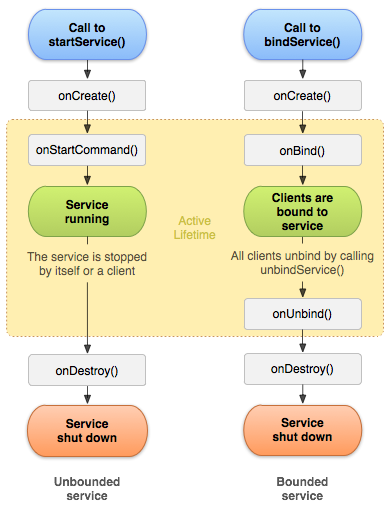
\includegraphics[width=10cm]{figures/service_lifecycle.png}
\caption{Ciclul de viață al unui serviciu}
\label{fig:service_lifecycle}
\end{figure}

\textbf{Content Provider}\\
Un content provider este o componentă care oferă acces la un set de date structurate, cum ar fi, de exemplu, contactele. Aceste componente încapsulează datele și oferă mecanisme pentru a defini chestiuni de securitate. Utilizarea lor este atunci când se dorește să se ofere acces la datele oferite de un proces unui alt proces.
Modul de lucru cu această componentă este similar într-o oarecare măsură cu lucrul cu o bază de date. Pentru a primi date se fac interogări, iar pentru a parcurge datele folosim un cursor.\\

\textbf{Broadcast Receiver}\\
Un broadcast receiver este o componentă care permite captarea și procesarea unor mesaje trimise de tip broadcast, trimise către oricine le poate înțelege și procesa.

Această componentă este declarată în AndroidManifest, acolo unde se specifică și ce mesaje poate să înțeleagă. Utilitatea lor este, de exemplu, de a „asculta” când s-a repornit telefonul, eventual pentru a porni alte aplicații și servicii.

\newpage
\subsection{API-uri Google}
Pe lângă paleta largă de obiecte pe care o pune la dispoziție prin sistemul Android, Google mai oferă și acces la servicii suplimentare care pot aduce mari îmbunătățiri aplicațiilor. Sunt servicii care scutesc dezvoltatorii de scris și testat cod, oferindu-le metode de a afișa hărți, de a introduce componente sociale în aplicații, de a construi jocuri noi, de a face procesări în cloud și nu numai.

Deși există o gamă largă de API-uri disponibile, vom discuta pe scurt doar despre unul dintre acestea, relevant în contextul acestei lucrări, Google Maps API.

\subsubsection{Google Maps API \cite{GoogleMapsAndroidAPI}}
API-ul Google Maps oferă dezvoltatorilor posibilitatea adăugării de hărți în aplicațiile lor. Aceste hărți pot conține toate funcționalitățile pe care le găsim în aplicația Google Maps, printre care și clădiri 3D, hărți ale clădirilor, imagini din satelit.

API-ul se ocupă în mod automat de tot ce înseamnă comunicarea cu serverele Google și cu afișarea hărții. Dezvoltatorul trebuie doar să implementeze funcționalitățile dorite peste cele de bază oferite deja de Google Maps. Dezvoltatorul poate, spre exemplu, să adauge propriul design harților, să modifice unghiul de vizualizare, să adauge linii, puncte sau alte elemente grafice pe diferite nivele (layers).

\newpage




\newpage
\section{Descrierea soluției implementate} \label{DescriereAplicatie}
Acest capitol va conține descrierea implementării aplicației, începând cu explicarea \textbf{interfeței vizuale} a aplicației și continuând cu explicarea \textbf{funcționalității} din fundal (aflare poziție GPS, detectare pași, măsurare pași, algoritm dead reckoning).

\subsection{Interfața} \label{DescriereInterfata}
Aplicația conține o \textbf{activitate} principală care oferă acces către mai multe \textbf{fragmente}. Fiecare fragment va oferi utilizatorului final o funcționalitate din cele descrise la început, în obiective.

Toate fragmentele sunt construite de către activitatea principală și păstrate în memorie. Acestea nu ocupă foarte multă memorie și deoarece sunt deja construite viteza cu care se deschid este una foarte bună, ele având deja toate datele necesare inițializate.

În continuare vor fi descrise fragmentele în ordinea apariției lor în meniul de navigație care apare din partea stângă (numit în cadrul Android \textit{NavigationDrawer}). Acest meniu arată așa cum este surprins în Figura \ref{fig:navigation_drawer}.

\begin{figure}[!htb]
\minipage{0.45\textwidth}
  \centering
  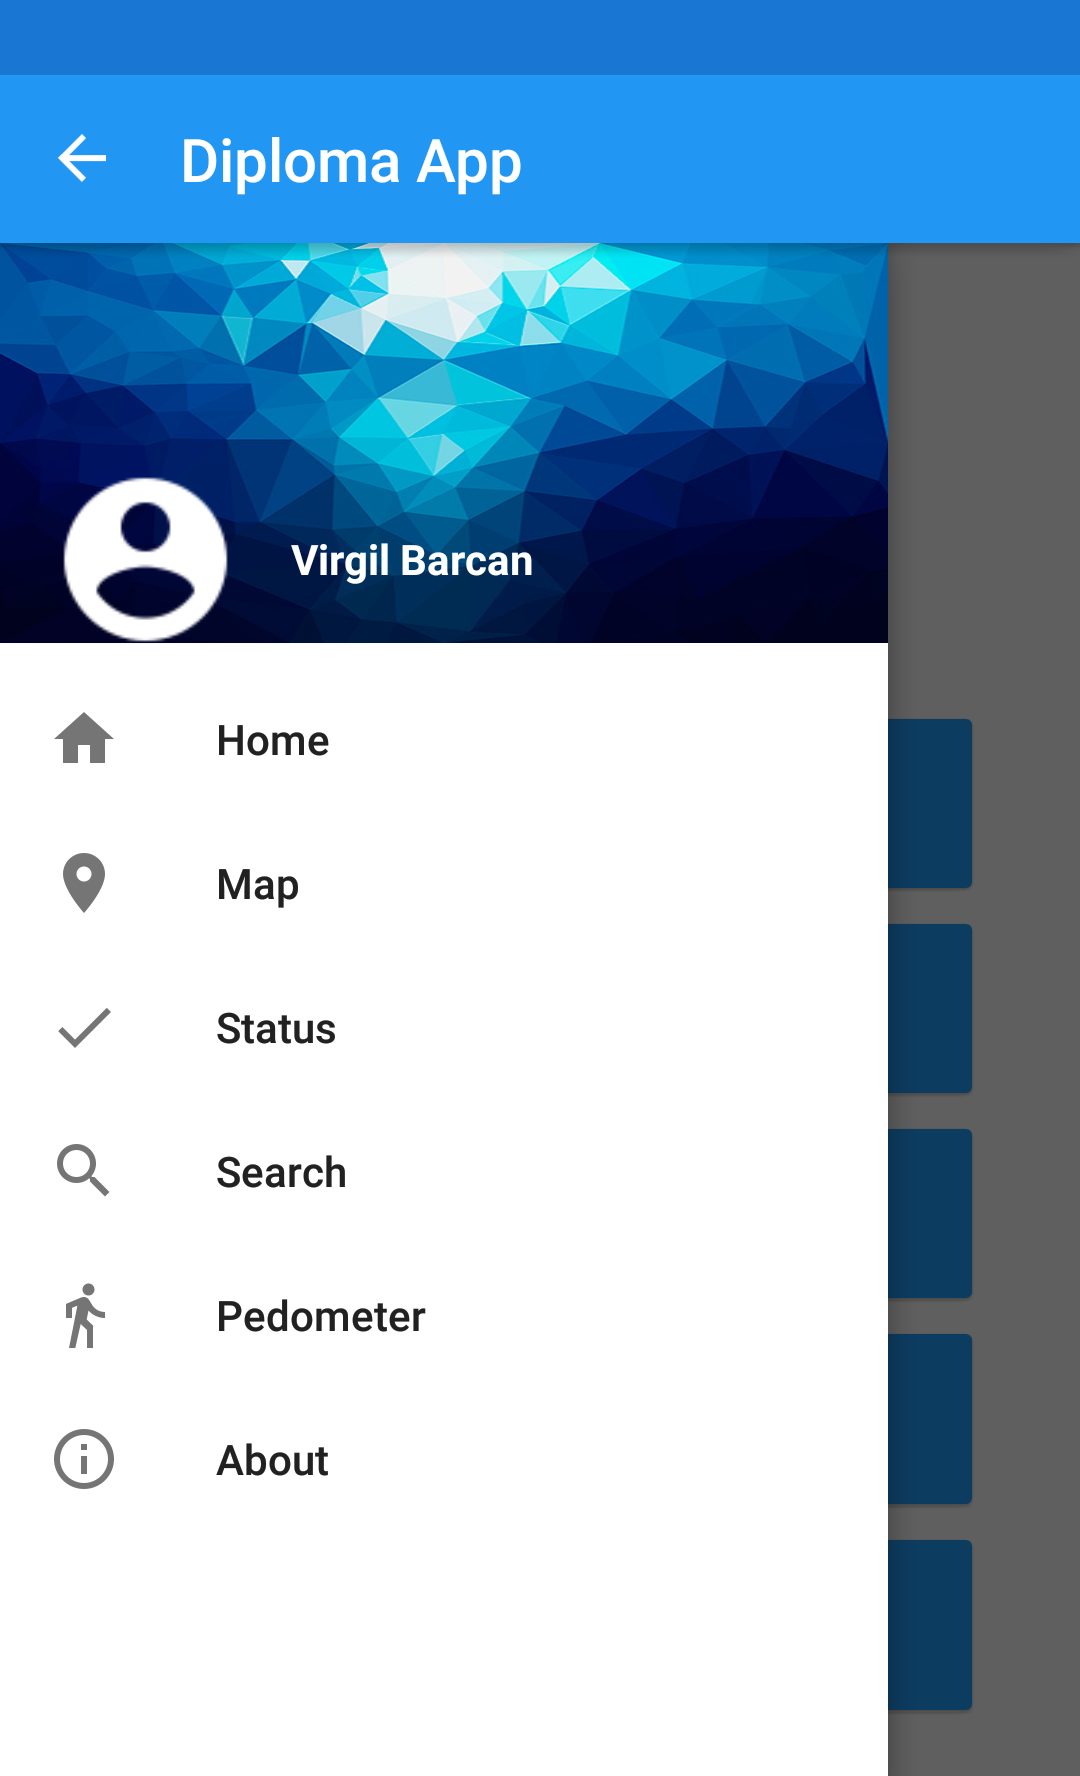
\includegraphics[width=5cm]{figures/navigation_drawer.png}
  \caption{NavigationDrawer}
  \label{fig:navigation_drawer}
\endminipage\hfill
\minipage{0.45\textwidth}%
  \centering  
  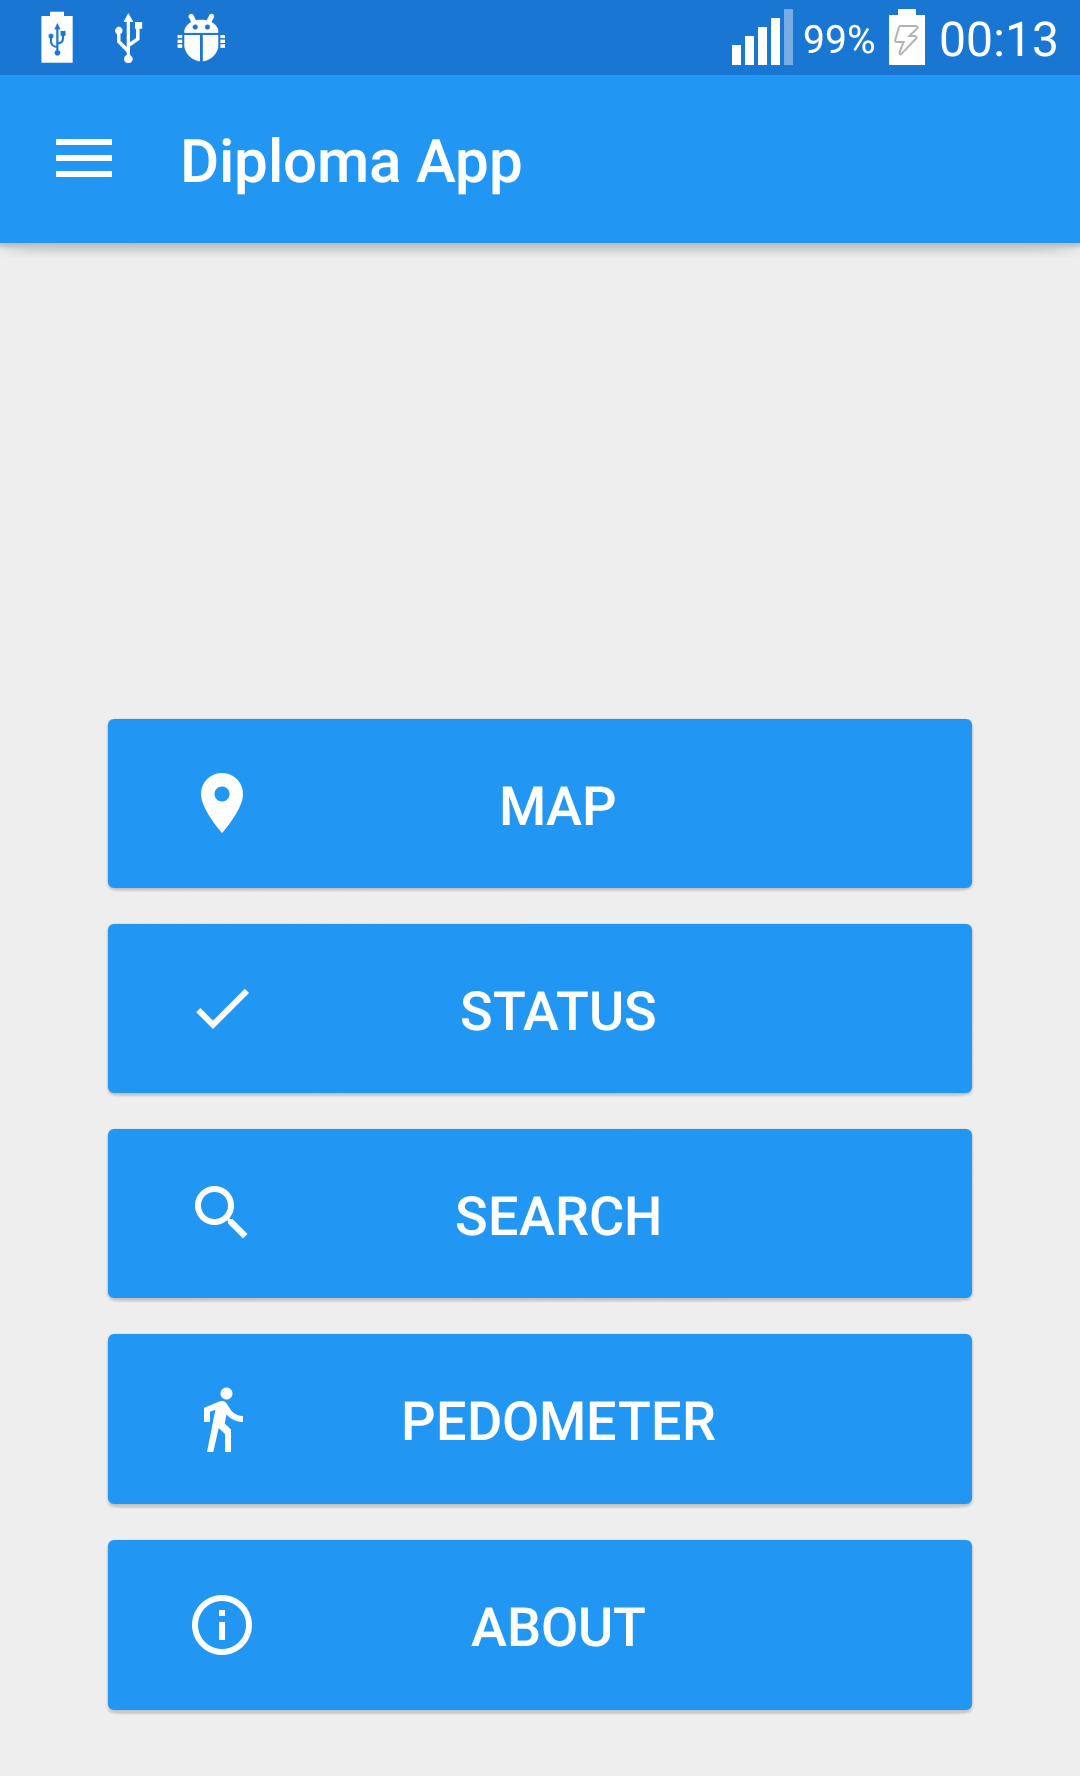
\includegraphics[width=5cm]{figures/fragment_home.png}
  \caption{Fragment Home}
  \label{fig:fragment_home}
\endminipage
\end{figure}

\begin{itemize}  
\item \textbf{Fragment Home}:\\
Acest fragment va oferi utilizatorului butoane prin care să navigheze în restul aplicației. Aceste butoane sunt prezente și în meniul din partea stângă, însă acesta este ascuns la deschiderea aplicației și de aceea a fost necesară implementarea unui fragment care să ofere aceeași funcționalitate. Modul în care arată acest fragment este surprins în Figura \ref{fig:fragment_home}.

\item \textbf{Fragment Map}:\\
Acest fragment este probabil cel mai important din întreaga aplicație, el fiind locul în care se văd clar rezultatele algoritmului din fundal. Acest fragment afișează poziția curentă, fie ea poziție GPS sau poziție calculată de algoritmul de dead reckoning, așa cum poate fi văzut în Figura \ref{fig:fragment_map}.

În cazul în care utilizatorul se deplasează, se va afișa și calea parcursă de acesta, bazată pe datele oferite de algoritmul de dead reckoning, care va fi explicat în secțiunea următoare.

Tot în acest fragment se afișează și eventualele puncte de interes căutate de către utilizator. Pentru punctele de interes selectate de către utilizator se afișează, la selectare, numele, așa cum poate fi văzut în Figura \ref{fig:fragment_map_interest_point}.

\begin{figure}[!htb]
\minipage{0.45\textwidth}
  \centering
  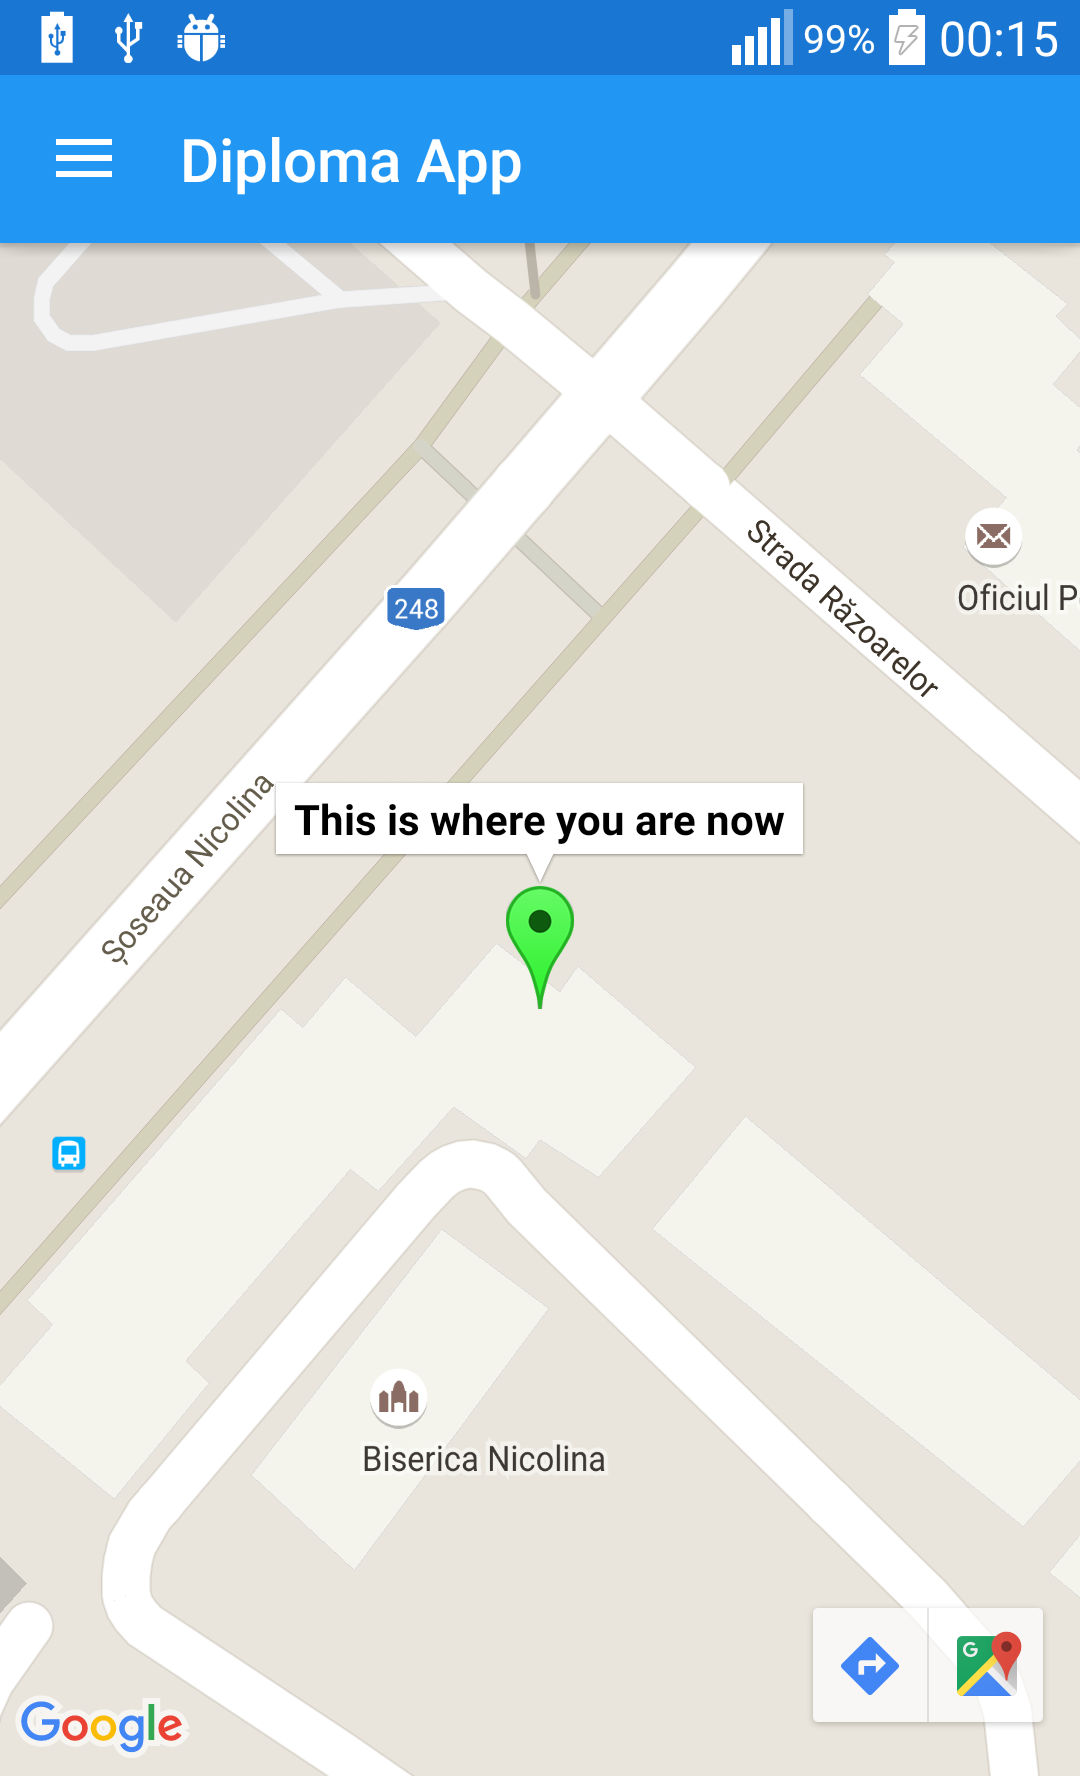
\includegraphics[width=5cm]{figures/fragment_map.png}
  \caption{FragmentMap - Locația curentă}
  \label{fig:fragment_map}
\endminipage\hfill
\minipage{0.45\textwidth}%
  \centering  
  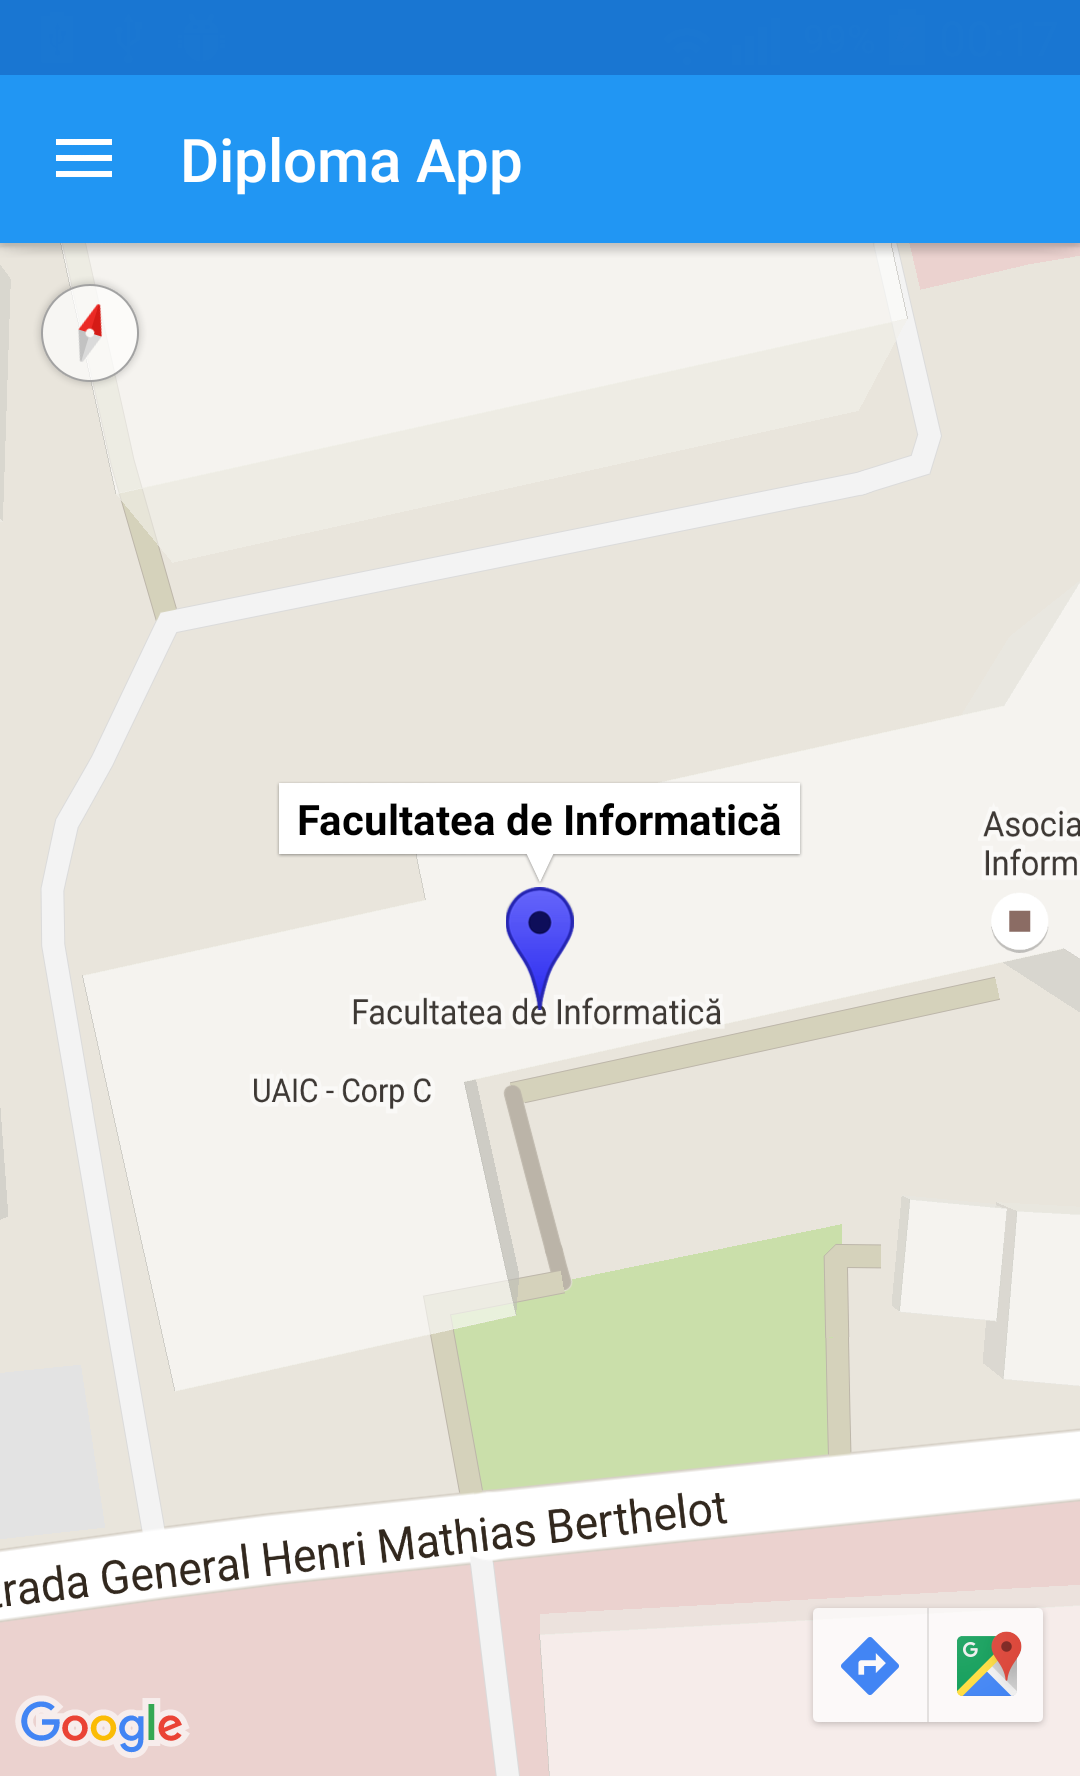
\includegraphics[width=5cm]{figures/fragment_map_interest_point.png}
  \caption{FragmentMap - Afișare punct de interes}
  \label{fig:fragment_map_interest_point}
\endminipage
\end{figure}

\item \textbf{Fragment Status}:\\
Acest fragment este util în special pentru faza de testare sau pentru cei curioși de cum variază diferiții parametri ai aplicației pe parcursul rulării acesteia.

În acest fragment se afișează valorile curente obținute de la senzori, cum ar fi acuratețea GPS-ului, locația GPS curentă și altele, cum se poate observa în Figura \ref{fig:fragment_status}.

\begin{figure}[!htb]
\minipage{0.45\textwidth}
  \centering
  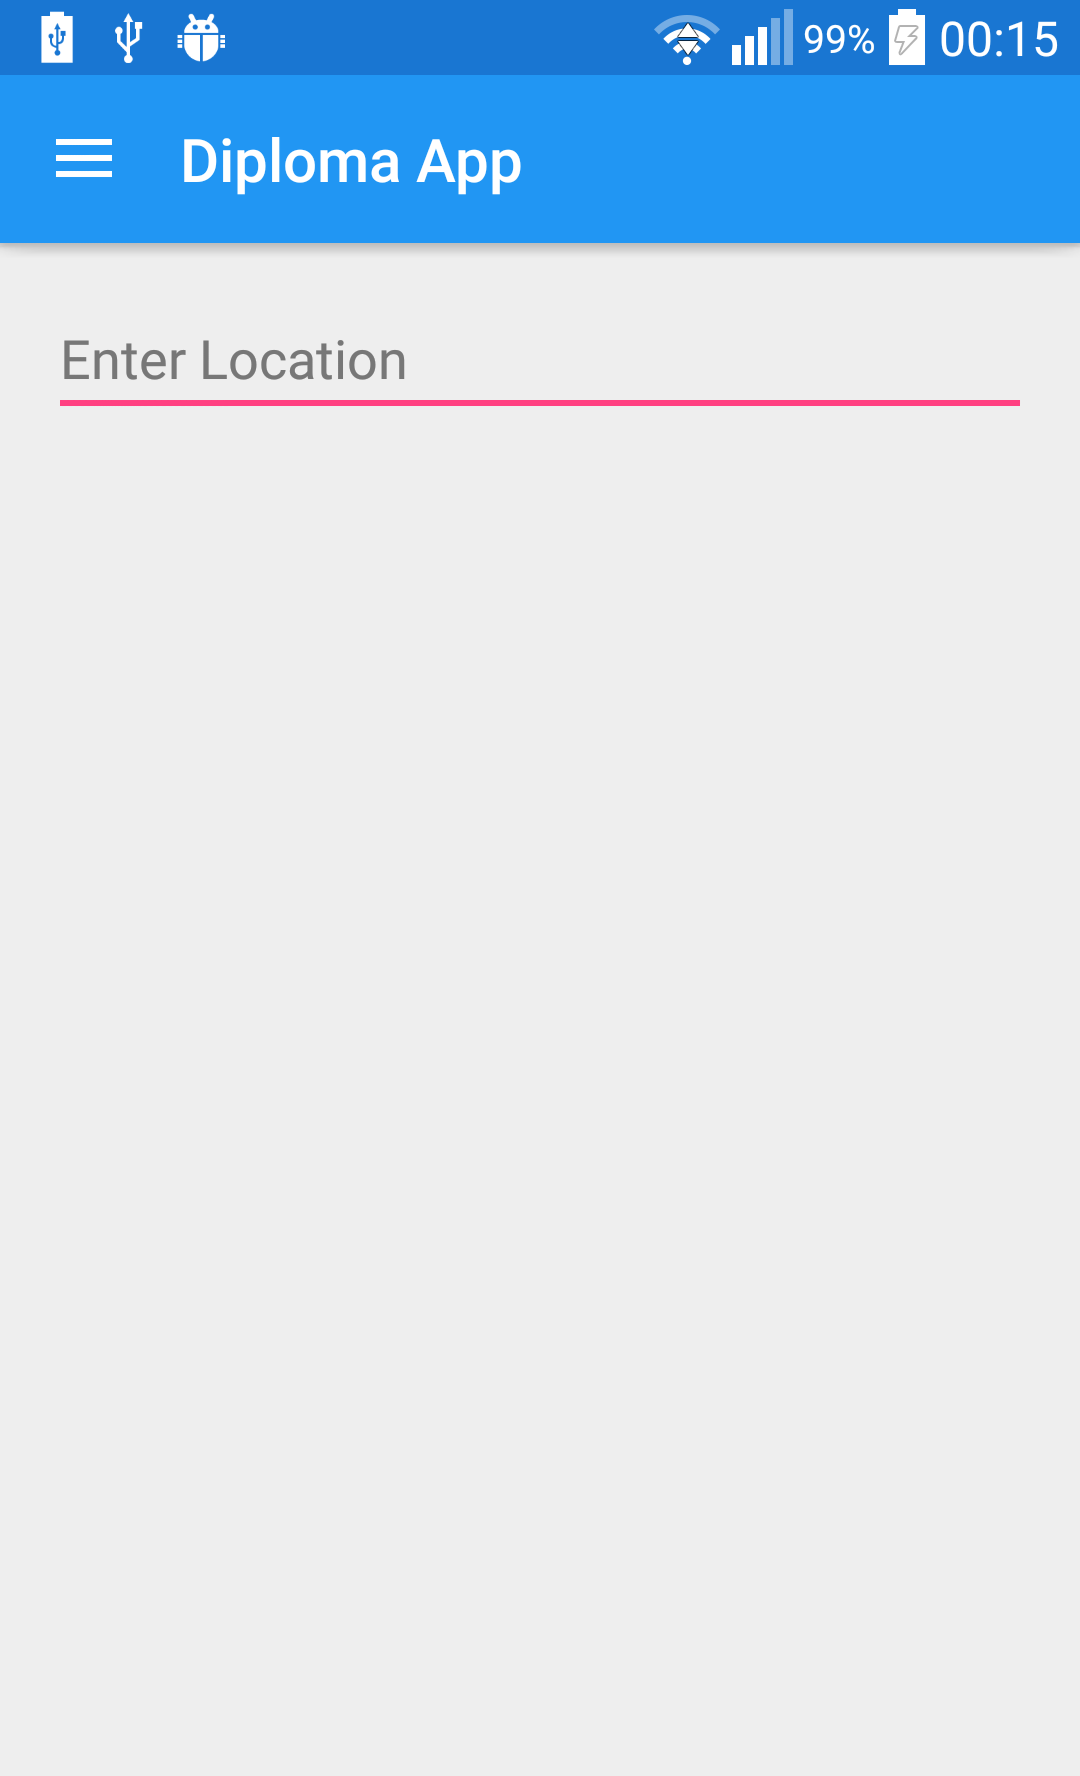
\includegraphics[width=5cm]{figures/fragment_search1.png}
  \caption{FragmentSearch - Ecran inițial}
  \label{fig:fragment_search1}
\endminipage\hfill
\minipage{0.45\textwidth}%
  \centering  
  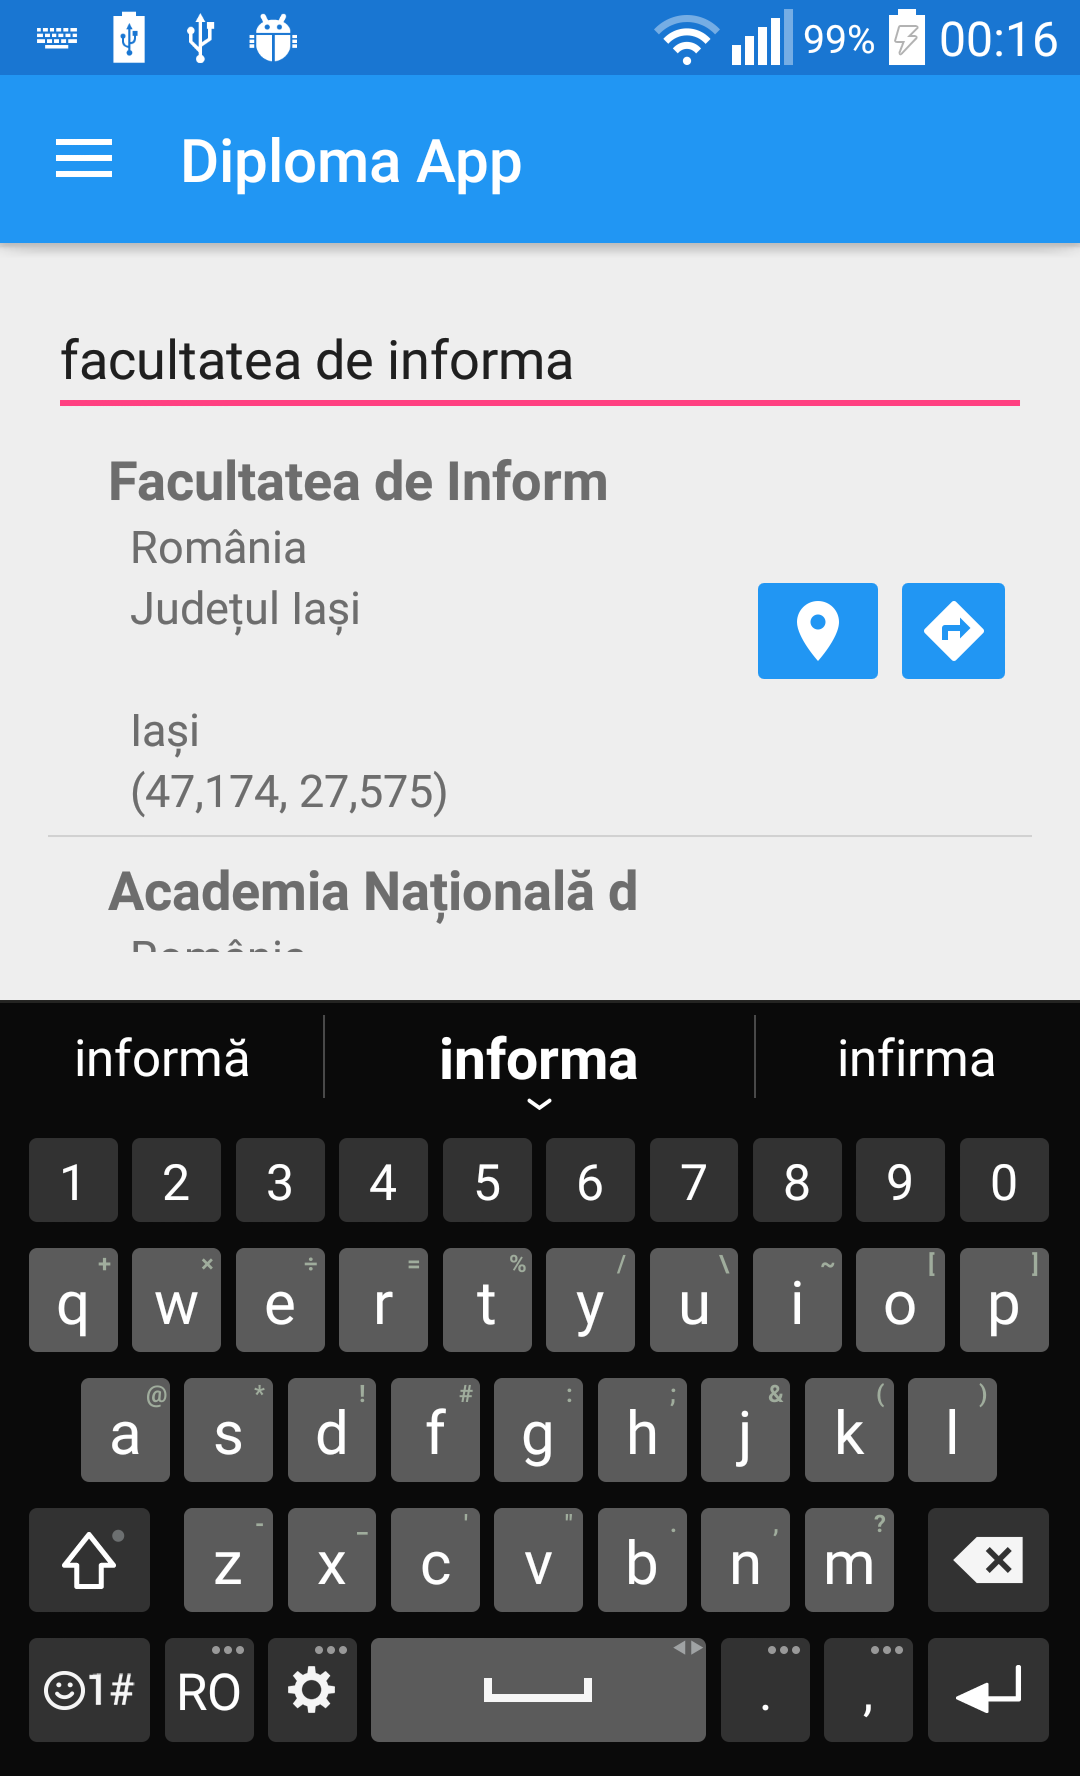
\includegraphics[width=5cm]{figures/fragment_search2.png}
  \caption{FragmentMap - Introducere text}
  \label{fig:fragment_search2}
\endminipage
\end{figure}

\item \textbf{Fragment Search}:\\
Acest fragment apare doar pentru a oferi utilizatorului posibilitatea căutării și vizualizării unor puncte de interes. Se vor putea construi și rute de la locația curentă către punctul selectat.

Utilizatorul trebuie să introducă numele punctului căutat. După ce vor fi scrise minim trei caractere, aplicația va căuta zece locații care să fie cele mai relevante și le va afișa în listă. Pentru fiecare astfel de element al listei se vor afișa și două butoane, unul de afișare pe hartă (cel din stanga) și unul de calculare a unei rute (cel din dreapta), așa cum se observă în Figurile \ref{fig:fragment_search1} și \ref{fig:fragment_search2}.


\begin{figure}[!htb]
\minipage{0.45\textwidth}
  \centering
  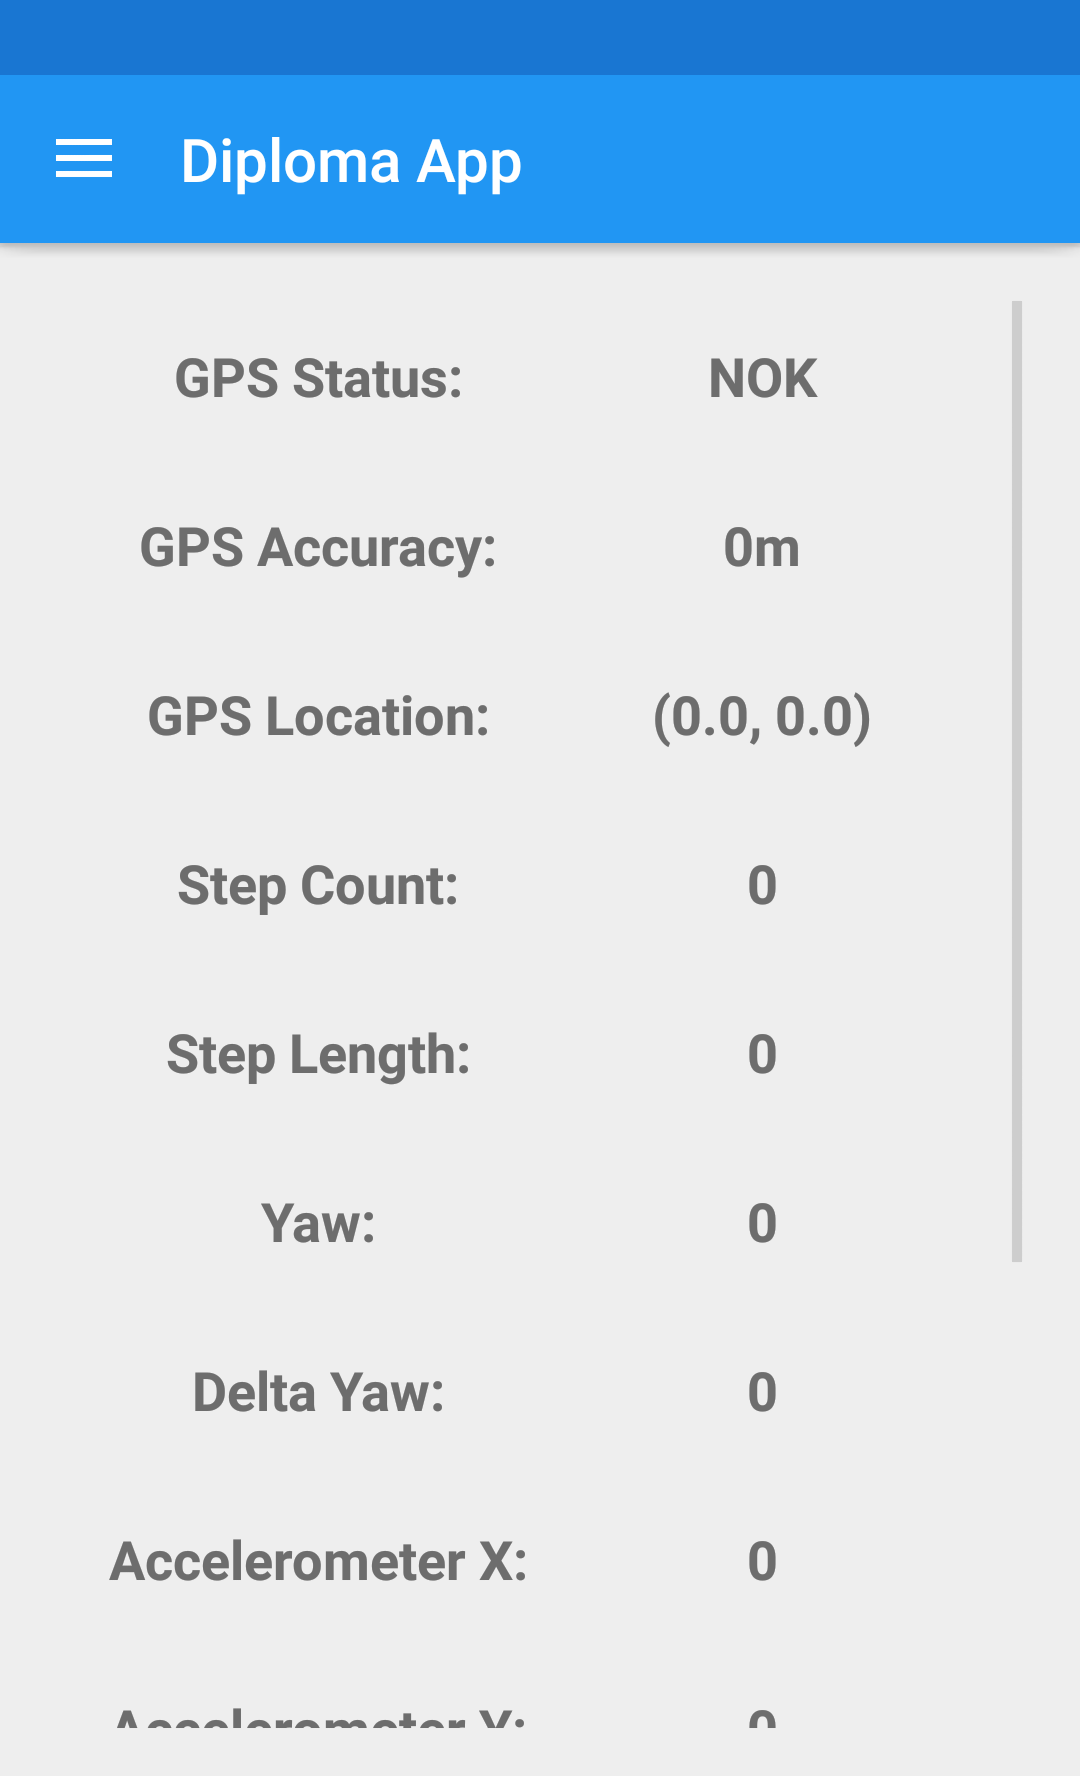
\includegraphics[width=5cm]{figures/fragment_status.png}
  \caption{FragmentStatus}
  \label{fig:fragment_status}
\endminipage\hfill
\minipage{0.45\textwidth}%
  \centering  
  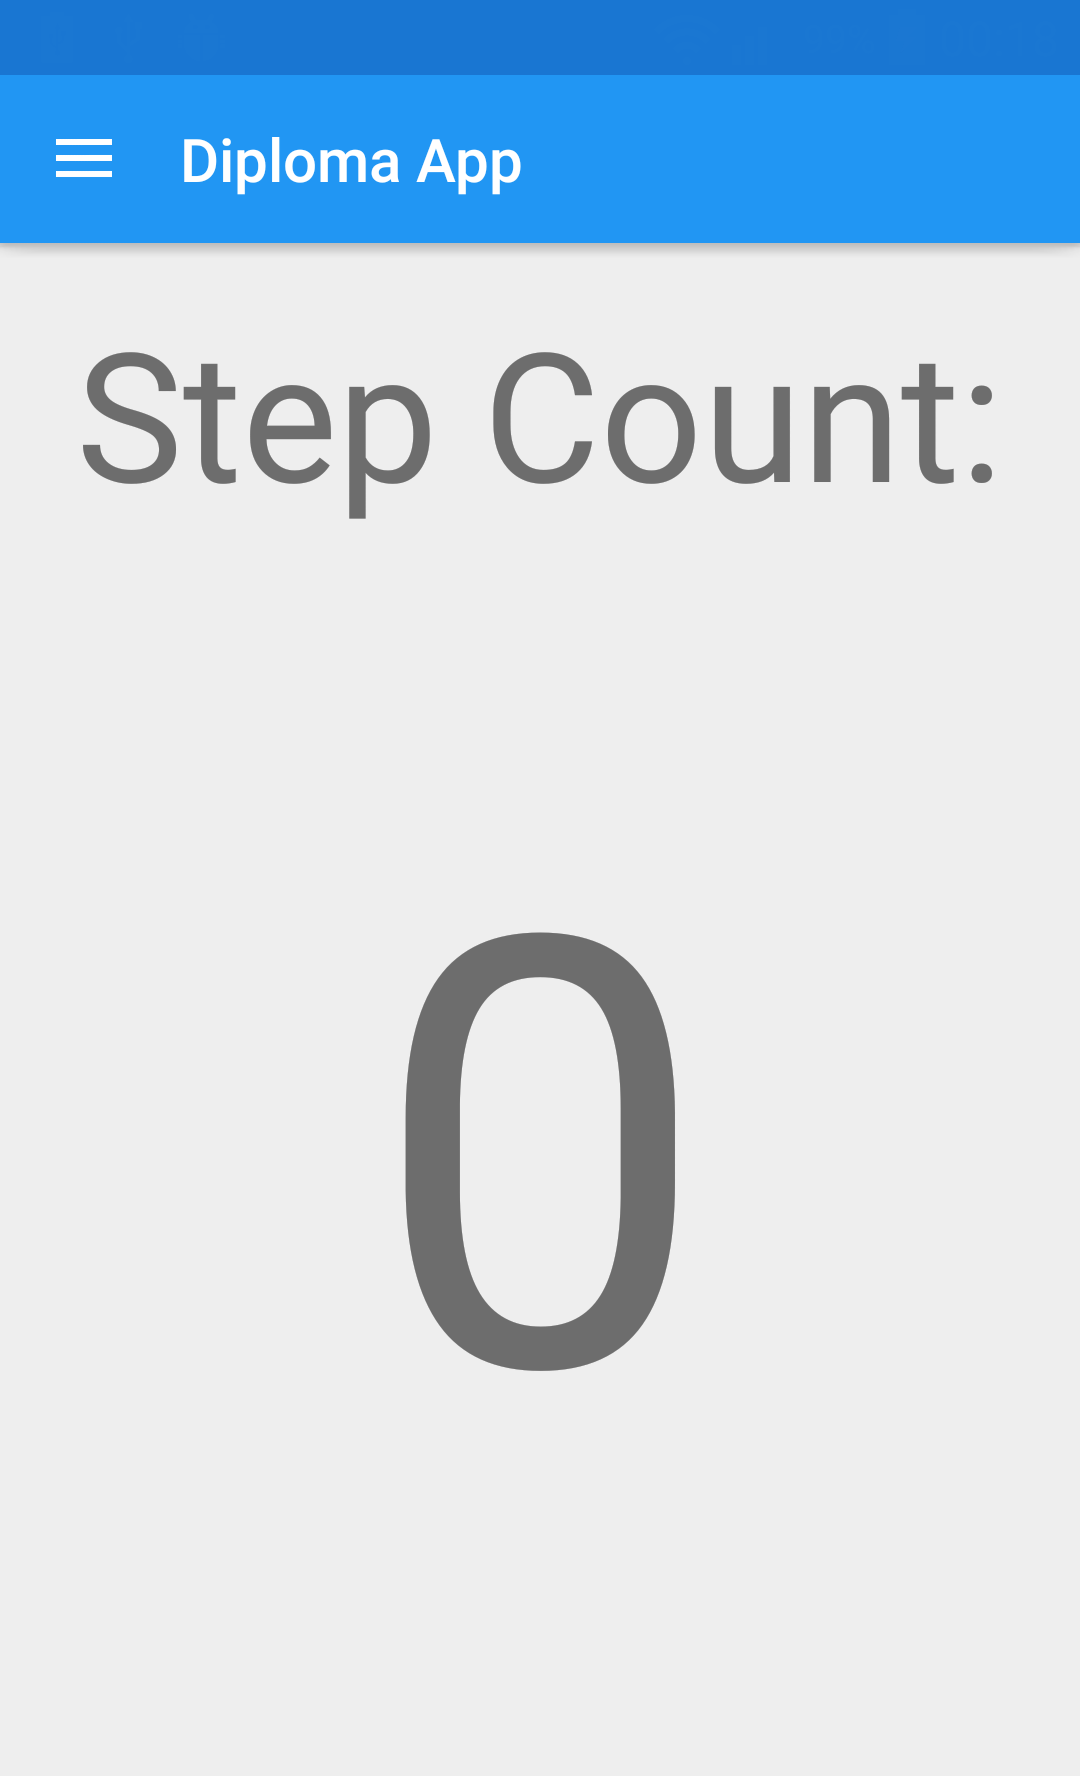
\includegraphics[width=5cm]{figures/fragment_pedometer.png}
  \caption{FragmentPedometer}
  \label{fig:fragment_pedometer}
\endminipage
\end{figure}


\item \textbf{Fragment Pedometer}:\\
Acest fragment poate fi util atunci când utilizatorul dorește doar să știe câți pași a făcut. Aici îi vor fi afișați toți pașii făcuți de când a început ziua. Acest fragment are o interfață simplistă, el existând doar pentru a apropia aplicația de zona de fitness. Interfața este cea din Figura \ref{fig:fragment_pedometer}.

\item \textbf{Fragment About}:\\
Acest fragment conține scurte detalii despre mine și despre aplicație, el nu face parte din lista fragmentelor relavante, așa cum sunt cele de mai sus.

\end{itemize}

\newpage
\subsection{Implementarea} \label{DescriereImplementare}
Implementarea aplicației s-a făcut având în vedere un consum cât mai redus de baterie, printr-o utilizare cât mai eficientă a resurselor. De aceea am luat decizia de a ascunde funcționalitățile „mari” în spatele unor module care să poată fi referențiate de mai multe obiecte, dar create doar o dată. Astfel de module sunt: \textbf{DeadReckoning} și \textbf{LocationHandler}. 

Modulul DeadReckoning este cel în care se calculează, bazat pe datele de la modulul de detecție al pașilor și al lungimii acestora, plus cele de la detectorul de schimbare a orientării față de nord, cunoscând poziția inițială, poziția curentă. Vom explica mai jos exact cum se face acest lucru.

Modulul LocationHandler este cel în care se face „ascultarea” poziției GPS curente, precum și a statusului acestui senzor (dacă este sau nu suficient de precisă poziția pentru a fi luată în considerare).

În rândurile următoare vom explica modul în care lucrează modulul de DeadReckoning (împreună cu modulele de care el depinde). 

\subsubsection{Dead Reckoning} \label{DeadReckoning}
Această clasă are un dublu comportament, unul de subiect și unul de observator (din perspectiva pattern-ului \textit{Observer}). El „ascultă” schimbările detectate de către detectorul de pași sau de către detectorul de schimbare a orientării și reacționează. Concret, detectorul de schimbare a orientării notifică faptul că avem un unghi nou față de nord iar clasa DeadReckoning stochează acest unghi actualizat. Detectorul de pași notifică atunci când detectează că un pas s-a făcut și clasa DeadReckoning foloște ultimul unghi primit de la detectorul de orientare împreună cu lungimea estimată a pasului pentru a calcula, având o ultimă poziție GPS, noile coordonate.

Descriu în continuare modul în care se face detecția pașilor, partea de orientare fiind obținută prin utilizarea unui modul extern obținut de la \cite{dsensor}.

Primul pas este colectarea datelor de la senzori. Datele primite de la senzori sunt stocate în interiorul clasei care ascultă evenimentele. Atunci când avem date pentru accelerația liniară, gravitație (ambele derivate din accelerația obținută de la accelerometru) și câmp magnetic, intrăm în procedura de transformare a sistemului de coordonate al datelor din cel local, descris în Figura \ref{fig:axis_device}, în cel global, descris în Figura \ref{fig:axis_globe}. Având datele în acest format, garantăm că putem detecta pașii indiferent de modul în care utilizatorul ține dispozitivul. Acesa poate să il țină în mână în orice poziție, în buzunar, etc. Algoritmul reușeste să detecteze pașii atât timp cât dispozitivul nu este supus unor alte mișcări, independent de mișcările utilizatorului.

Detecția pașilor se face analizând forma undei generate. Așa cum se poate observa din Figura \ref{fig:walk_wave}, unda rezultată în urma efectuării unor pași are o formă relativ în care găsim zone de accelerație minimă și zone de accelerație maximă. Zonele de accelerație minimă apar atunci când persoana atinge pământul cu călcâiul, iar cele de accelerație maximă atunci când piciorul este ridicat și în balans către pasul următor. Există numeroase studii în legătură cu mersul uman, \cite{HumanWalkAndRunParameters}, \cite{HumanGaitCycle}, \cite{WalkCycle}, însă ce este relevant pentru proiectul acesta este că putem detecta destul de simplu dacă un pas a fost sau nu făcut.

\begin{figure}[h]
\centering
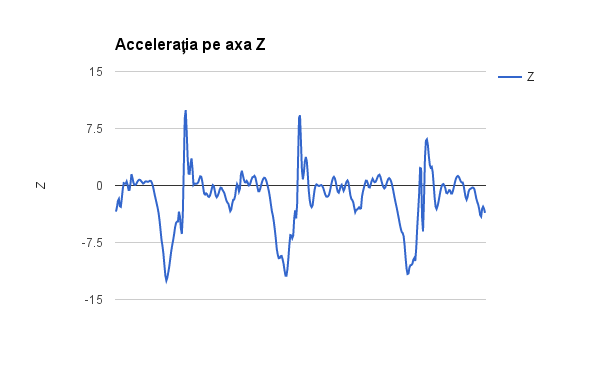
\includegraphics[width=10cm]{figures/walk_wave.png}
\caption{Unda accelerometru pentru trei pași}
\label{fig:walk_wave}
\end{figure}

Pentru a detecta dacă un pas a fost sau nu făcut, urmărim fie apariția unei scăderi a accelerației către un minim local, fie apariția unei creșteri a accelerației către un maxim local. Diferența în valoare absolută între minim și maxim trebuie să se încadreze într-o marjă pentru ca un pas să fie numărat. Aceste marjă este, la început, una generală, însă după calibrare ea va fi una care se va „plia” după utilizator.

Putem descrie algoritmul de detecție a pașilor foarte simplu, numărăm câte schimbări minim-maxim, maxim-minim au avut loc. Numărul de pași este suma celor două valori aproximată prin adaos (preferăm să numărăm un pas în plus).

După detectarea pasului, trebuie estimată distanța parcursă. Pentru a face asta, folosim formula descrisă de Harvey Weinberg în \cite{HarveyWeinberg}: lungimea unui pas k, $\rho_{k}$, este $\rho_{k} = K \sqrt[4]{A_{max}^{(k)} + A_{min}^{(k)}}$, unde $A_{max}^{(k)}$ este valoarea maximă a accelerației în timpul celui de-al k-lea pas, $A_{min}^{(k)}$ este valoarea minimă a accelerației în timpul celui de-al k-lea pas, iar $K$ este o constantă dependentă de utilizator. Această constantă este definită ca raportul dintre lungimea reală parcursă de utilizator și lungimea estimată (folosind doar radicalul). Pentru a o afla avem o fază de calibrare. Altfel, această valoare este una predefinită și erorile pot fi destul de mari.

Având la dispoziție informația că s-a realizat un pas și știind și lungimea acestuia, modulul de detecție a pașilor poate anunța modulul de dead reckoning.

Având la dispoziție date despre orientarea curentă și lungimea ultimului pas, pe lângă datele privind ultima poziție (latitudine, longitudine), algoritmul de dead reckoning va esima poziția curentă folosind Formula lui Vincenty, descrisă în \cite{VincentyFormulae}. Deși detaliile matematice sunt peste scopul acestei lucrări, este important de menționat ce poate face această formulă. 

Formula este folosită atât pentru aflarea distanței dintre două puncte aflate pe Pământ la coordonate date, cât și la aflarea coordonatelor unui punct destinație cunoscând coordonatele punctului de start, distanța parcursă și orientarea. Deși există soluții mai simple pentru această problemă (de exemplu, formula haversină \cite{HaversineFormula}), această soluție este una extrem de precisă: până la $0.5mm$ pentru distanță și $0.000015″$ pentru orientare. Deși există o variantă îmbunătățită a acestei formule, propusă de Charles Karney \cite{Karney2013}, acea metodă nu este atât de simplu de implementat. De mare ajutor în partea de implementare a fost biblioteca găsită pe Github, simplelatlng \cite{simplelatlng}.

Având la dispoziție datele despre poziția curentă calculată, modulul de dead reckoning va anunța toți observatorii, pentru ca aceștia să își modifice stările. De exemplu, FragmentMap va afișa un marker cu noua poziție, precum și linia care arată ruta dintre ultima poziție și cea curentă.


\subsubsection{Location Handler} \label{LocationHandler}
Clasa care se ocupă de locație este LocationHandler. Această clasă are o implementare similară cu cea a clasei DeadReckoning, în sensul că ea este și subiect și observator. 

Clasa ascultă notificările venite de la serviciul de locație al Android, implementând interfața LocationListener. Atunci când primește notificarea de locație schimbată, clasa verifică daca statusul serviciului era unul care să garanteze că datele sunt unele de încredere (acuratețe ridicată și 3D Fix pornit).

Dacă datele sunt de încredere, clasa notifică mai departe toți observatorii.

\newpage
\section{Testarea soluției implementate} \label{TestareAplicatie}
Testarea s-a făcut folosind un smartphone LG G2 dotat cu accelerometru, giroscop și magnetometru, pe lângă alți senzori.

Pentru testare se vor lua în calcul două chestiuni, performanța detectorului de pași și performanța sistemului per total. Pentru a evalua performanța detectorului de pași se vor face teste folosind detectorul standard de pași oferit de Google Fit, o brățară Jawbone și telefonul cu algoritmul prezentat în lucrare. Se vor face 100 de pași numărați și se vor verifica rezultatele celor trei.

Pentru a evalua performanța sistemului per total, se vor efectua două feluri de teste, ambele în aer liber. Se va aștepta conectarea GPS-ului, care va fi considerat referință. Se vor efectua teste în linie dreaptă și teste cu căi care să conțină manevre la stânga, respectiv dreapta, în forma unui dreptunghi. Se vor urma mereu aceleași căi și se va verifica dacă ruta oferită de GPS este aceeași cu ruta oferită de algoritm, ambele comparate cu ruta reală, cunoscută.


\newpage
\section{Discuții și muncă ulterioară} \label{DiscutiiMuncaUlterioara}
\section{Discuții} \label{Discutii}
TODO


\section{Muncă ulterioară} \label{MuncaUlterioara}
Aplicația prezentată este doar un prototip, ea nefolosind algoritmi deosebit de avansați. O primă chestiune de îmbunătățit este folosirea unei metode de genul unui filtru Kalman extins (unul extins deoarece datele nu respectă neapărat o condiție de liniaritate). Alte posibilități, așa cum au studiat și alții, ar fi acelea ale unor filtre de particule sau filtre probabiliste.

Merită încercată o astfel de îmbunătățire a algoritmului folosit pentru aducerea unui plus de performanță. Totuși, această folosire a unui algoritm performant aduce cu sine și un consum ridicat de baterie. O altă îmbunătățire ar fi, deci, găsirea unei soluții fie de a efectua calculele cât mai eficient, fie de a le face pe un alt dispozitiv, cum ar fi în cloud.

Printre alte îmbunătățiri ce ar putea fi aduse, deși nu neapărat aplicației în sine, ar fi încercarea de a cartografia clădiri mari din zona Iași, cum ar fi mall-urile sau universitatea. Aplicația poate avea un potențial uriaș în a ajuta elevii care doresc să se înscrie la facultate să găsească facultatea și, ulterior, sălile.

Probabil o altă arie ce ar putea deveni interesantă ar fi aceea a oferirii aplicației în parteneriat cu magazine mari (cum ar fi Carrefour sau Auchan) ca un asistent virtual pentru găsirea de produse/rafturi.

Desigur, una dintre cele mai importante utilizări ar putea fi găsită în zona Palas, în special în parcare. O eventuală cartografiere pe Google Maps, susținută de o îmbunătățire a aplicației, ar putea-o transforma în una de mare ajutor acolo.

Se mai pot aduce, desigur, și noi funcționalități, cum ar fi oferirea de sugestii de magazine care oferă reduceri sau oferirea de informații despre diferite zone din interiorul clădirilor (picturile din corpul A al Universității, de exemplu).

\newpage
\section{Concluzii} \label{Concluzii}
Din punctul meu de vedere această lucrare a fost un succes, obiectivele stabilite la începutul ei fiind atinse. Deși mai sunt lucruri de îmbunătățit, ideea în sine este una cu potențial, fapt dovedit de încercările Google de a cartografia cât mai multe clădiri (există posibilitatea trimiterii de hărți către ei, sistemul fiind unul deschis).

Munca la această lucrare a presupus o aprofundată cercetare a unor domenii dintre cele mai vaste: începând de la studiul senzorilor și continuând cu studiul sistemului GPS, al modului în care funcționează mersul uman, al modului în care se fac lucrurile în Android, și încheind cu studiul unor algoritmi dintre cei mai diverși: de la cei probabiliști la algoritmi de estimare sau de calculare deterministă.

Efortul depus a adus însă satisfacția de a pune o idee în practică, iar pentru asta eu sunt extrem de mulțumit.

Sper ca în perioada ce urmează să se insiste mai mult pe acest domeniu încă neexplorat suficient deoarece este clar că acesta este unul extrem de interesant și cu un potențial enorm de a aduce o îmbunătățire a calității călătoriilor.

\newpage
\addcontentsline{toc}{section}{Bibliografie}
%Paginile dedicate bibliografiei
\bibliography{inside_nav_bib}
\bibliographystyle{unsrt}
\nocite{*}

\end{document}
